\section{experimental evaluation}\label{sec:exp}
In this section, we conduct extensive experiments by comparing the proposed hash table design \voter, with several state-of-the-art GPU-based hash table approaches and one CPU-based concurrent hash table approach. 
Section~\ref{sec:exp:setup} introduces the experimental setup. 
Section~\ref{sec:exp:tune} presents a discussion on the sensitivity analysis of \voter.
In Sections~\ref{sec:exp:static} and \ref{sec:exp:dynamic}, we compare all approaches under the static and the dynamic experiments respectively.

\subsection{Experimental Setup}\label{sec:exp:setup}

\vspace{1mm}\noindent\textbf{Baselines.} We compare \voter with several state-of-the-art hash table implementations on both CPUs and GPUs. These implementations include the following:
\begin{itemize}
	\item \revise{\chash is a well-established CPU-based concurrent hash table that parallelizes a cuckoo hash \cite{li2014algorithmic}. }
	\item \cudpp is a popular CUDA primitive library containing the cuckoo hash table implementation published in~\cite{alcantara2009real}.  
	In our experiments we use the default setup of \cudpp, which automatically chooses the number of hash functions based on the data to be inserted.
	\item \revise{\warp is a state-of-the-art warp-centric approach for GPU-based hash tables \cite{junger2018warpdrive}. \warp employs a linear probe approach to handle hash collisions. }
	\item \megakv is a warp-centric approach for GPU-based key value store published in~\cite{zhang2015mega}. \megakv employs a cuckoo hash with two hash functions and
	it allocates a bucket for each hash value. 
	\item \slab is a state-of-the-art GPU-based dynamic hash table \cite{ashkiani2018dynamic}, which employs chaining and a dedicated memory allocator for resizing.
	%\item \google is an efficient CPU-based hash table implementation\footnote{https://github.com/sparsehash/sparsehash-c11/}. We choose the \emph{dense\_hash\_map} implementation since it provides the best efficiency.
	\item \voter is the approach proposed in this paper. 
\end{itemize}
We adopt the implementations of the compared baselines from their corresponding inventors.
\revise{The code for \voter is released~\footnote{https://github.com/pauline-ly/Dycuckoo}. 
Performance numbers for GPU-based solutions are calculated based purely on GPU run-time. The overhead of data transfer between CPUs and GPUs can be hidden by overlapping data transfer and GPU computation, as proposed by MegaKV \cite{zhang2015mega}. Since this technique is orthogonal to the approaches proposed in our paper, we focus solely on GPU computation. 
} 
%For \megakv, we note that its intra-block synchronization could lead to inconsistency issue as well as a large number of insertion failures, especially when the filled factor is high.  
%Thus, we revise its code by replacing the intra-block synchronization with atomicExch to resolve the race condition. The adoption of atomicExch preserves the design principle of \megakv for \emph{not} locking the entire bucket for updates. Moreover, it leads to less insertion failures and similar performance against its original implementation. 

%Note that we do not compare with the dynamic GPU hash approach proposed in \cite{ashkiani2018dynamic} for two major reasons. First, we cannot obtain the original implementation from its authors. Second, the approach devises a dedicated memory allocator other than cudaMalloc. A dedicated allocator will improve the performance but add complexity the system. Additionally, it needs to occupy a large memory in advance and is not transparent to other GPU applications.
%In contrast, our proposed approach only uses native allocator supported. 
%We do not compare with \cite{breslow2016horton} since it only improves \megakv marginally using a more costly insertion process.

\begin{table}[t]
	\caption{The datasets used in the experiments.}
	\vspace{-1.5em}
	\label{table:exp_data_sets}
	\centering
	%\begin{tabular}{|c|c|c|c|}
	%	\hline
	%	Datasets & KV pairs & Unique keys & Max Duplicates \\ \hline
	%	\dstwitter &50,876,784 & 44,523,684&4\\ \hline
	%	\dsreddit & 48,104,875 & 41,466,682 &2 \\ \hline
	%	\dstpch &50,000,000 & 45,159,880&4\\ \hline
	%	\dsali &10,000,000 & 4,583,941&14\\ \hline
	%	\dsrandom & 100,000,000& 100,000,000& 1 \\ \hline
	%\end{tabular}
\begin{tabular}{|c|c|c|}
	\hline
	Datasets & KV pairs & Unique keys\\ \hline
	\dstwitter &50,876,784 & 44,523,684\\ \hline
	\dsreddit & 48,104,875 & 41,466,682 \\ \hline
	\dstpch &50,000,000 & 45,159,880\\ \hline
	\dsali &10,000,000 & 4,583,941\\ \hline
	\dsrandom & 100,000,000& 100,000,000 \\ \hline
\end{tabular}
\end{table}



\vspace{1mm}\noindent\textbf{Datasets.} We evaluate all compared approaches using several real world datasets. The summary of the datasets can be found in Table~\ref{table:exp_data_sets}.
\begin{itemize}
	\item \dstwitter: Twitter is an online social network where users perform the actions \emph{tweet}, \emph{retweet}, \emph{quote}, and \emph{reply}.
	We crawl these actions for one week through the Twitter stream API\footnote{https://dev.twitter.com/streaming/overview} for the following trending topics: US president election, 2016 NBA finals and Euro 2016. The dataset contains 50,876,784 KV pairs.
	\item \dsreddit: Reddit is an online forum where users perform the actions \emph{post} and \emph{comment}. We collect all Reddit \emph{comment} actions in May 2015 from \emph{kaggle}~\footnote{https://www.kaggle.com.reddit/reddit-comments-may-2015} and query the Reddit API for \emph{post} actions during the same period. The dataset contains 48,104,875 KV pairs. 
 	\item \dstpch: Lineitem is a synthetic table generated by the TPC-H benchmark\footnote{https://github.com/electrum/tpch-dbgen}. We generate  100,000,000 rows of the lineitem table and combine the \emph{orderkey}, \emph{linenumber} and \emph{partkey} column as keys. 
	\item \dsrandom: Random is a synthetic dataset generated from a normal distribution. We have deduplicated the data and generated 100,000,000 KV pairs.  
	\item \dsali: Databank is a PB-scale data warehouse that stores Alibaba customer behavior data for 2017. Because of confidentiality concern, we sample 10,000,000 transactions and the dataset contains 4,583,941 encrypted customer IDs as KV pairs.
\end{itemize}






%



\vspace{1mm}\noindent\textbf{Static Hashing Comparison (Section~\ref{sec:exp:static}).}
We evaluate \formal{insert} and \formal{find} performance among all compared approaches under a static setting. 
We insert all KV pairs from the datasets and then issue 1 million random search queries. 



%\begin{figure*}[ht]
%	\begin{minipage}{0.3\linewidth}\centering
%		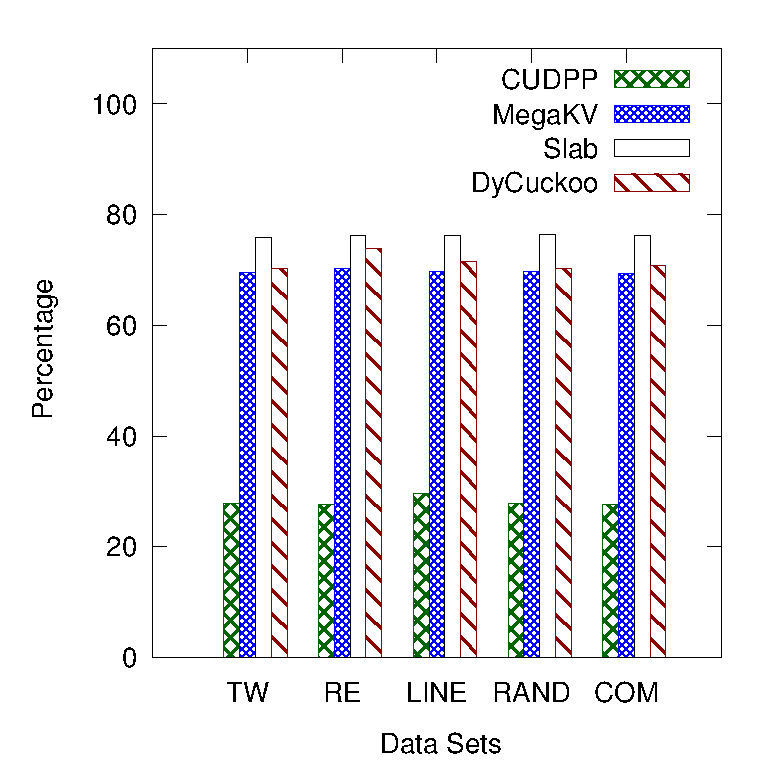
\includegraphics[width=\linewidth]{pic/static-profi/warp.eps}
%		\centerline{Warp Efficiency}
%	\end{minipage}
%	\hfill
%	\begin{minipage}{0.3\linewidth}\centering
%		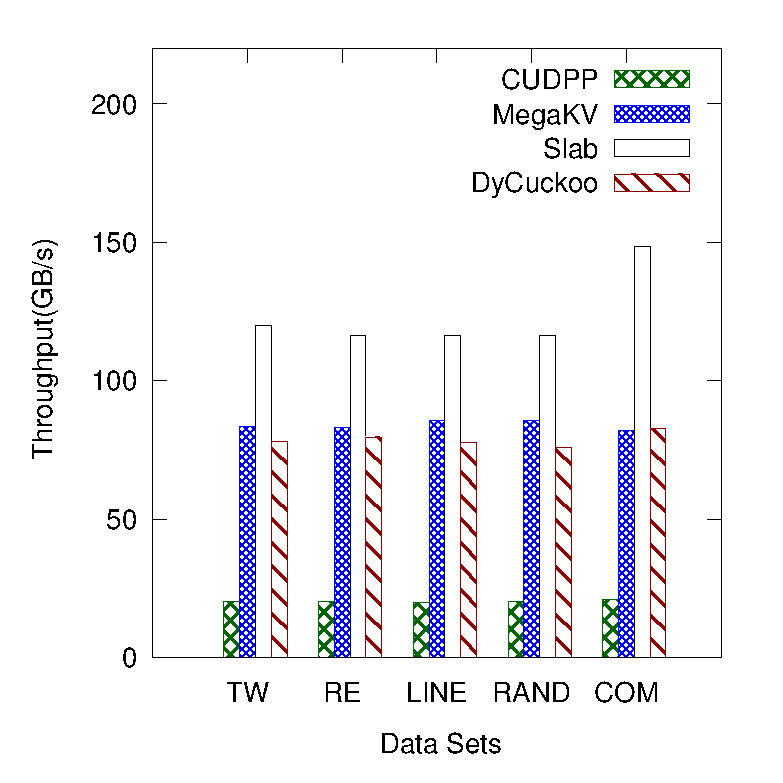
\includegraphics[width=\linewidth]{pic/static-profi/L2-read.eps}
%		\centerline{Cache Utilization}
%	\end{minipage}
%	\hfill
%	\begin{minipage}{0.3\linewidth}\centering
%		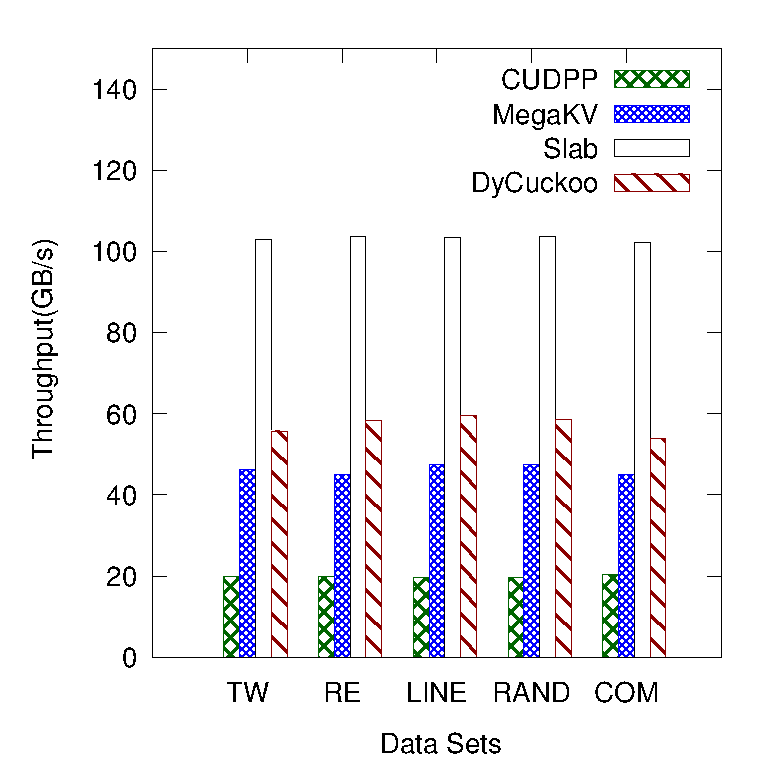
\includegraphics[width=\linewidth]{pic/static-profi/memory-read.eps}
%		\centerline{Memory Bandwidth Utilization}
%	\end{minipage}
%	\caption{GPU profiling results for static hashing comparison.}
%	\label{fig:static:profile}
%\end{figure*}


\vspace{1mm}\noindent\textbf{Dynamic Hashing Comparison (Section~\ref{sec:exp:dynamic}).}
We generate workloads under the dynamic setting by batching hash table operations.
We then partition the datasets into batches of $1$ million insertions. 
For each batch, we augment $1$ million \formal{find} operations and $1 \cdot r$ million \formal{delete} operations,
where $r$ is a parameter for controlling insertions and deletions.
After exhausting all the batches, we rerun the batches by swapping the \formal{insert} and \formal{delete} operations in each batch. 
In other words, we issue $1$ million deletions of the keys inserted, 1 million \formal{find} operations and $1 \cdot r$ million \formal{insert} operations.
We then evaluate the performance of all compared GPU approaches except for \cudpp and \warp as they do not support deletions. 
We also exclude the CPU approach as it is significantly slower than the GPU-based approaches according to Figure~\ref{fig:static-all}. 
Since \megakv does not provide dynamic resizing, we double/half the memory usage followed by rehashing all KV pairs as a resizing strategy if the corresponding filled factor falls out of the specified range. 
Moreover, if an insertion failure is found for a compared approach, we trigger its resizing strategy.

\begin{table}[t]
	\centering
	\caption{Parameters in the experiments}
	\vspace{-1.5em}
	\label{tbl:parameters}
	\begin{tabular}{|c|c|c|}
		\hline
		\textbf{Parameter} & \textbf{Settings} & \textbf{Default} \\ \hline
		Filled Factor	$\theta$  & 70\%, 75\%, 80\%, 85\%, 90\% & 85\% \\ \hline
		Lower Bound $\alpha$ & 20\%, 25\%, 30\%, 35\%, 40\% & 30\% \\ \hline
		Upper Bound	$\beta$  & 70\%, 75\%, 80\%, 85\%, 90\% & 85\% \\ \hline
		Ratio $r$ & 0.1, 0.2, 0.3, 0.4, 0.5 & 0.2 \\ \hline
		Batch Size & 2e5, 4e5, 6e5, 8e5, 10e5 & 10e5 \\ \hline
	\end{tabular}
\end{table}

\vspace{1mm}\noindent\textbf{Parameters.}
We vary the parameters when comparing \voter with the baselines.
Here, $\alpha$ represents the lower bound for filled factor $\theta$ for all compared approaches, $\beta$ is the respective upper bound, and $r$ is the ratio of insertions over deletions in a processing batch. 
The parameter settings are listed in Table~\ref{tbl:parameters}. For all experiments, we use \emph{million operations/seconds} (Mops) as a metric to measure the performance of all compared approaches.

\revise{
\vspace{1mm}\noindent\textbf{Experiment Environment.}
We conduct all experiments on an Intel Xeon E5-2682 Server equipped with an NVIDIA Tesla P100-PCIe GPU. Evaluations are performed using CUDA 9.1 on Centos 7.2. The optimization level (-O3) is applied for compiling all programs.
}


\begin{figure}[t]
	\begin{minipage}{0.48\linewidth}\centering
		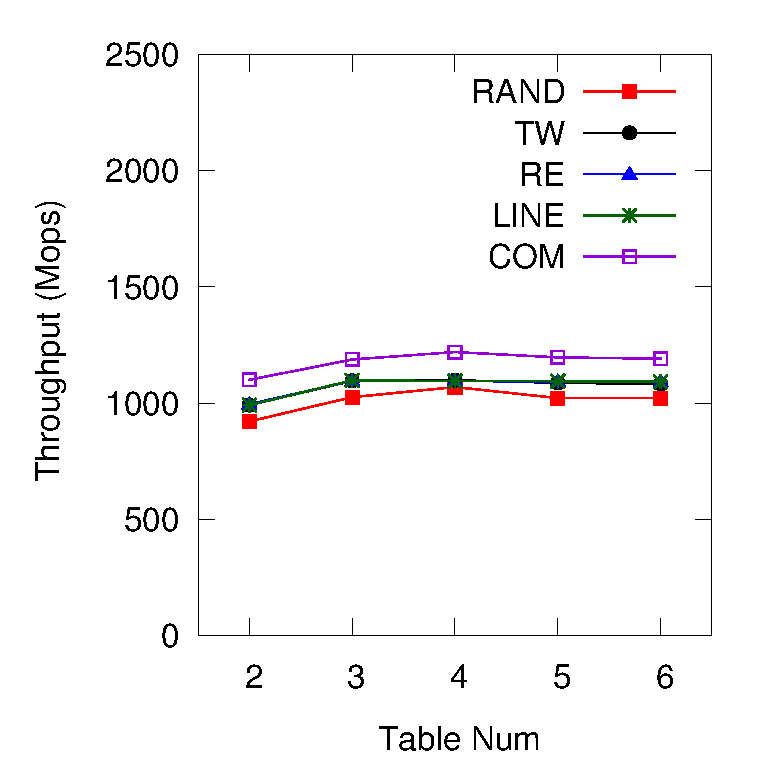
\includegraphics[width=\linewidth]{pic/tunning/tunning-insert.eps}
		\centerline{\formal{insert}}
	\end{minipage}
	\hfill
	\begin{minipage}{0.48\linewidth}\centering
		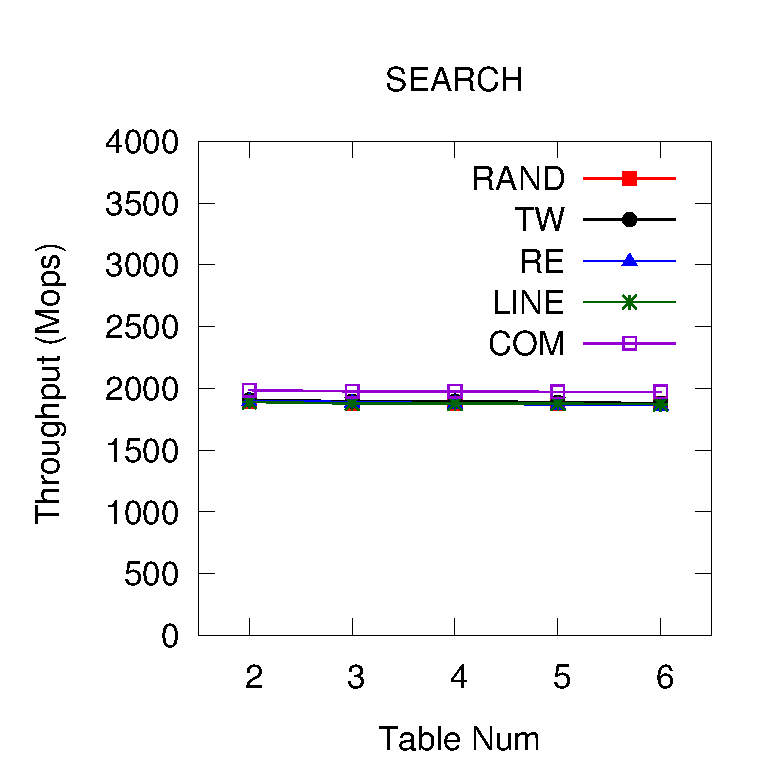
\includegraphics[width=\linewidth]{pic/tunning/tunning-search.eps}
		\centerline{\formal{find}}
	\end{minipage}
	\caption{\revise{Throughput of \voter for varying the number of hash tables.}}
	\label{fig:vary-table}
\end{figure}
%
\begin{figure}[t]
	\begin{minipage}{0.48\linewidth}\centering
		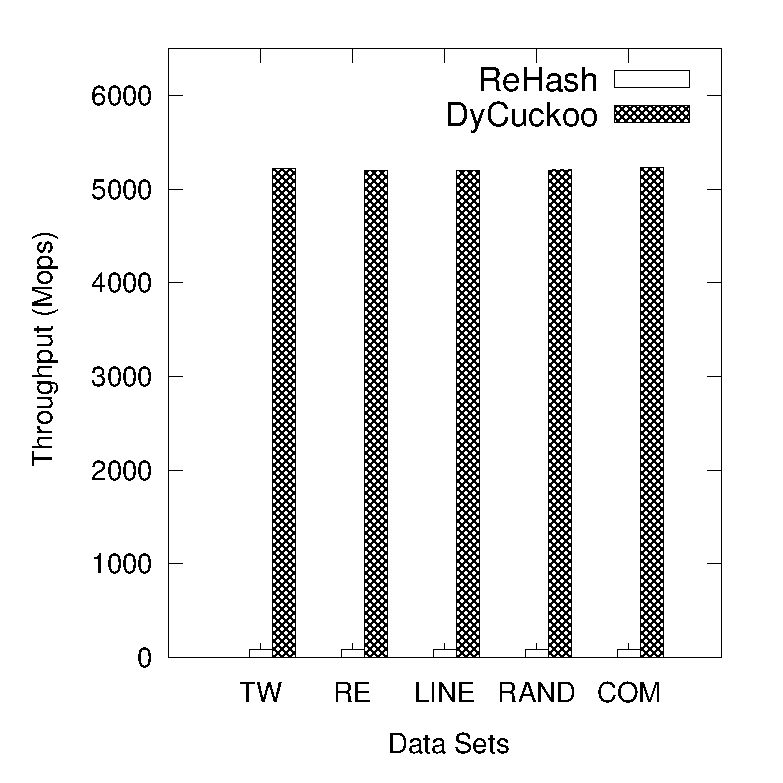
\includegraphics[width=\linewidth]{pic/compare/upsize.eps}
		\centerline{\formal{upsize}}
	\end{minipage}
	\hfill
	\begin{minipage}{0.48\linewidth}\centering
		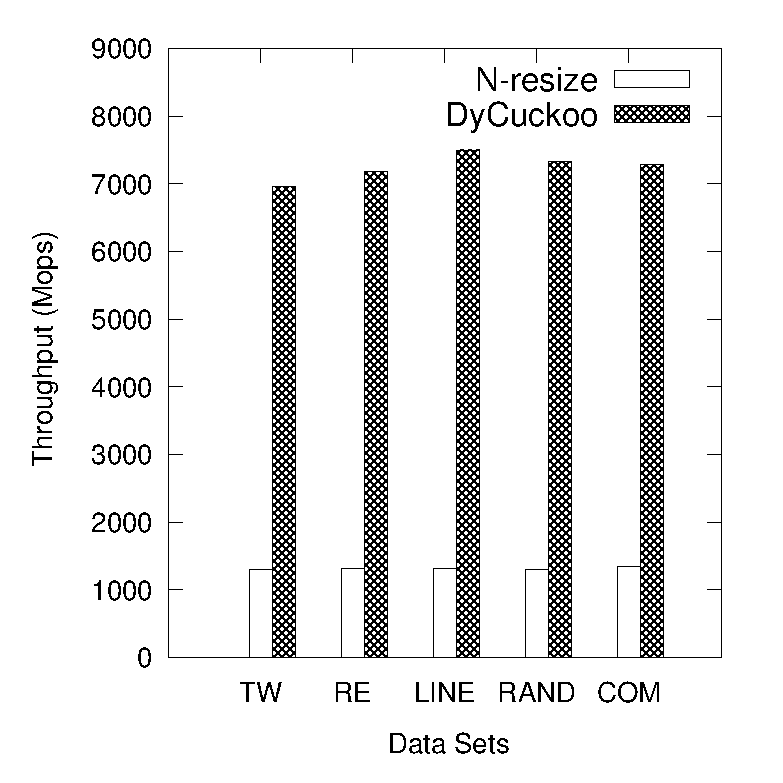
\includegraphics[width=\linewidth]{pic/compare/downsize.eps}
		\centerline{\formal{downsize}}
	\end{minipage}
	\caption{\revise{Throughput of subtable resize.}}
	\label{fig:resize}
\end{figure}

%\begin{table}
 %\centering
 %\caption{The number bucket accessed of subtable resize.}
 %\begin{tabular}{|c|c|c|c|c|c|c|}
 %\hline  &  & \dstwitter & \dsreddit &  \dstpch & \dsali &  %\dsrandom \\
  %\hline
  %\multirow{2}*{UPSIZE} & Dcuckoo& 1133 & 1024 & 1062 & 1081 &  1021 \\
  %\cline{2-7}
  %~ &N-resize & 31,4444 & 31,4485 & 31,4528 & 31,4326 & 31,4453 \\
  %\hline
  %\multirow{2}*{DOWNSIZE} & Dcuckoo& 70,1055 & 70,4030 & 70,7677 & 70,2058 &  70,6265 \\
  %\cline{2-7}
  %~ &N-resize & 138,6990 & 138,8938 & 139,0672 & 138,7547 & 138,7034 \\
  %\hline
 %\end{tabular}
%\end{table}


\begin{table}[b]
	\centering
	\caption{\revise{The number bucket accessed for subtable resizing (x1000).}}
	\vspace{-1.5em}
	\label{tab:buckets}
	\begin{tabular}{|c|c|c|c|c|}
		\hline  
		& \multicolumn{2}{c|}{UPSIZE} & \multicolumn{2}{c|}{DOWNSIZE} \\ \hline
		& \voter & Rehash & \voter & Rehash \\ \hline
%		\dstwitter & 4740536 & 5642137 & 628271 & 628759 \\ \hline
%		\dsreddit & 4739004 & 5653021 & 628338 & 628779 \\ \hline
%		\dstpch& 4745519 &  5659083 & 628279 & 628946\\ \hline
%		\dsali& 4735274 & 5648726 & 628346 & 628938 \\ \hline
%		\dsrandom& 4731278 & 5646791 & 628421 & 628879 \\ \hline		
		\dstwitter & 4740 & 5642 & 628 & 629 \\ \hline
		\dsreddit & 4739 & 5653 & 628 & 629 \\ \hline
		\dstpch& 4746 &  5659 & 628 & 629\\ \hline
		\dsali & 4735 & 5649 & 628 & 629 \\ \hline
		\dsrandom & 4731 & 5647 & 628 & 629 \\ \hline
	\end{tabular}
\end{table}

\subsection{Sensitivity Analysis}\label{sec:exp:tune}

\vspace{1mm}
\noindent\textbf{Varying the number of tables.}
A key parameter affecting the performance of \voter is the number of hash tables chosen. For the static scenario, we present the throughput performances of \formal{insert} and \formal{find} for a varying number of hash tables, as shown in Figure~\ref{fig:vary-table}, while fixing the entire structure's memory space ensure a default filled factor of $\theta$. 
\formal{insert} increases its throughput with more hash tables, since there are more alternative locations to relocate KV pairs. 
\revise{However, performance slightly degrades with more than four hash tables. This is because the total size of the allocated memory is fixed,
and thus each table becomes smaller for more tables. This leads to more evictions for some overly occupied tables, thus slightly degrading the performance.
Another interesting observation is that we achieve the best performance with the \dsali dataset. This is because \dsali has the smallest ratio of unique keys (Table~\ref{table:exp_data_sets}). Inserting an existing key is equivalent to an update operation, which has better performance than inserting a new key.}
The throughput of \formal{find} remains constant for additional hash tables as the two-layer cuckoo hashing guarantees a maximum of two look ups for \formal{find}. In the remainder part of this section, we fix the number of hash tables at four.

\vspace{1mm}
\noindent\textbf{Resizing analysis.}
To validate the proposed resizing strategy's effectiveness, we compare it with rehashing. 
For upsizing, we initialize \voter with all data and set the filled factor as the default upper bound of $85\%$. We perform a one time upsizing, i.e., we upsize one subtable, and then compare our resizing strategy against rehashing all subtable entries by reinserting the entries using Algorithm~\ref{algo:insert}.
The setup for downsizing is a mirror image of upsizing, except with an initial filled factor set as the default lower bound of $30\%$. 
\revise{We record the number of buckets accessed to process all resizing strategies in Table~\ref{tab:buckets}. First, downsize accesses less buckets than that of upsize as there are smaller number of KV pairs to be moved for downsize (total size of the allocated table is fixed). Furthermore, \voter and rehash access similar number of buckets for downsize as the table is mostly empty at the filled factor of 30\%. Second, \voter accesses smaller number of buckets than that of rehash in the upsize scenario. This is because the tables are almost filled for upsize at 85\%, which leads to more cuckoo evictions for rehash whereas no eviction required for \voter. In Figure~\ref{fig:resize}, we also measure the throughput of both methods as the number of KV pairs to be moved over the time to complete resizing. The throughput advantage of \voter cannot be explained solely by the smaller number of buckets accessed for resizing. In fact, \voter does not need to lock any buckets for upsizing and only needs to lock a small number of buckets for downsizing when eviction, whereas rehash needs to lock every accessed buckets. The experimental results confirm the superiority of our proposed resizing strategy.}

\begin{figure}[t]
	\begin{minipage}{0.48\linewidth}\centering
		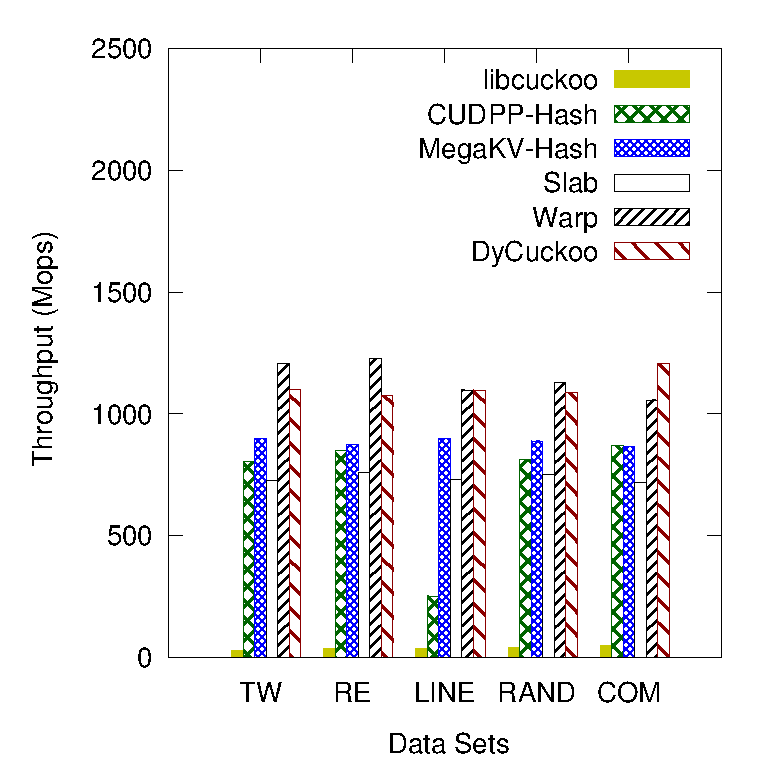
\includegraphics[width=\linewidth]{pic/static/static_insert.eps}
		\centerline{\formal{insert}}
	\end{minipage}
	\hfill
	\begin{minipage}{0.48\linewidth}\centering
		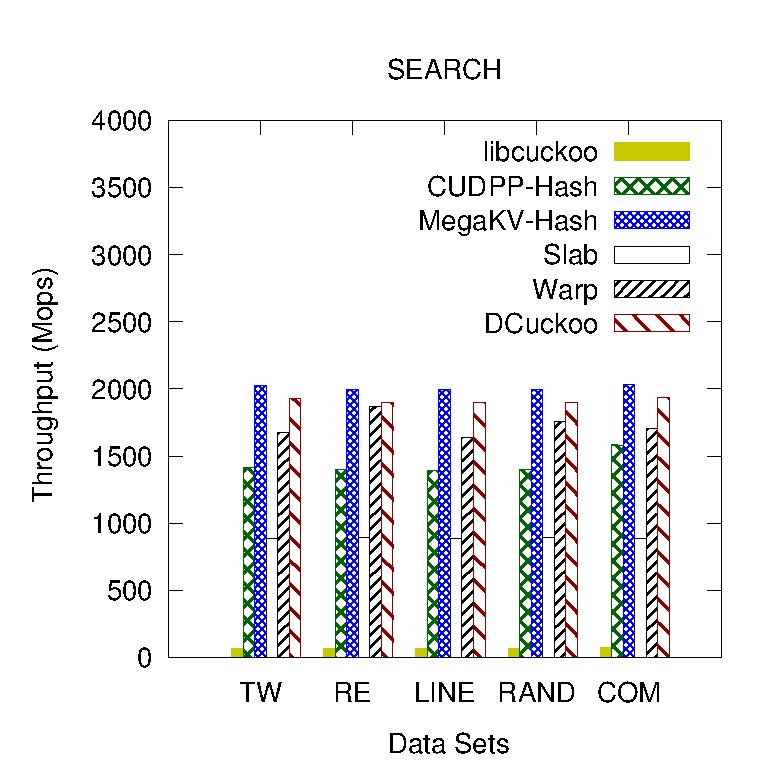
\includegraphics[width=\linewidth]{pic/static/static_search.eps}
		\centerline{\formal{find}}
	\end{minipage}
	\caption{\revise{Throughput of all compared approaches under the static setting.}}
	\label{fig:static-all}
\end{figure}
%
\begin{figure}[t]
	\begin{minipage}{0.48\linewidth}\centering
		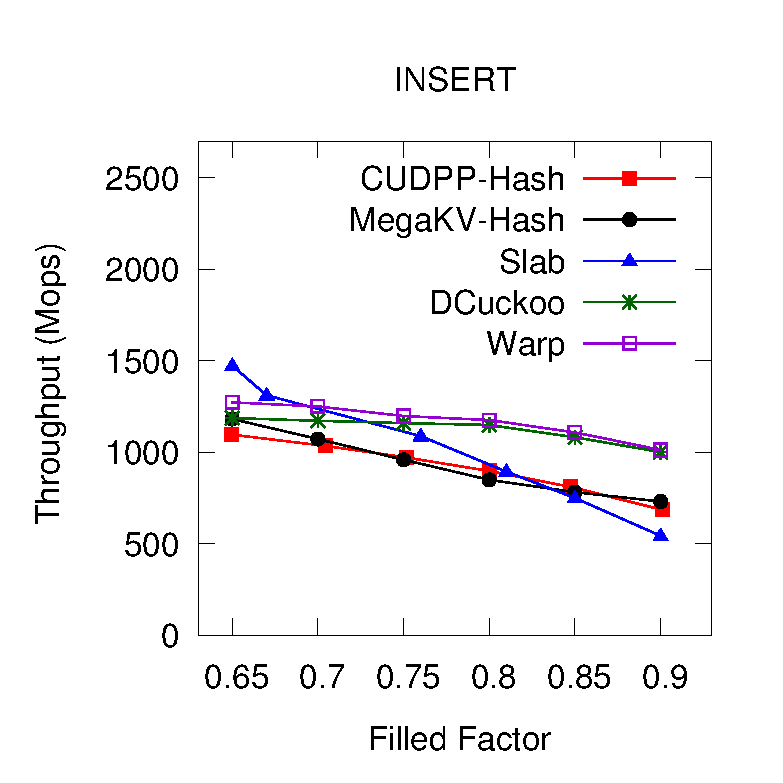
\includegraphics[width=\linewidth]{pic/static-load_factor/random/insert.eps}
		\centerline{\formal{insert}}
	\end{minipage}
	\hfill
	\begin{minipage}{0.48\linewidth}\centering
		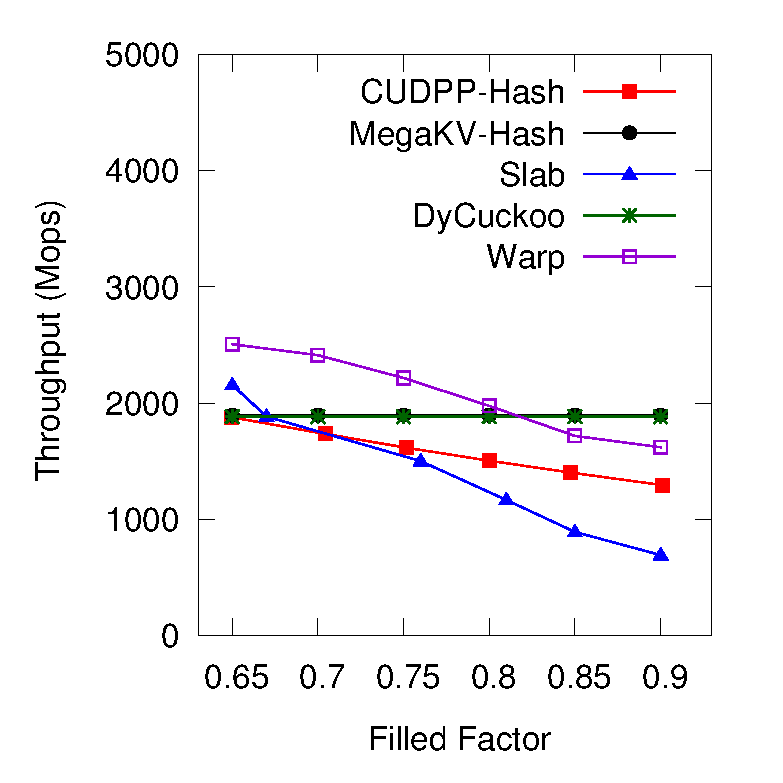
\includegraphics[width=\linewidth]{pic/static-load_factor/random/search.eps}
		\centerline{\formal{find}}
	\end{minipage}
	\caption{\revise{Throughput of all compared approaches for varying the filled factor against the \dsrandom dataset.}}
	\label{fig:static-filled-factor}
\end{figure}

\iffalse
\begin{figure}[h]
	\begin{minipage}{0.48\linewidth}\centering
		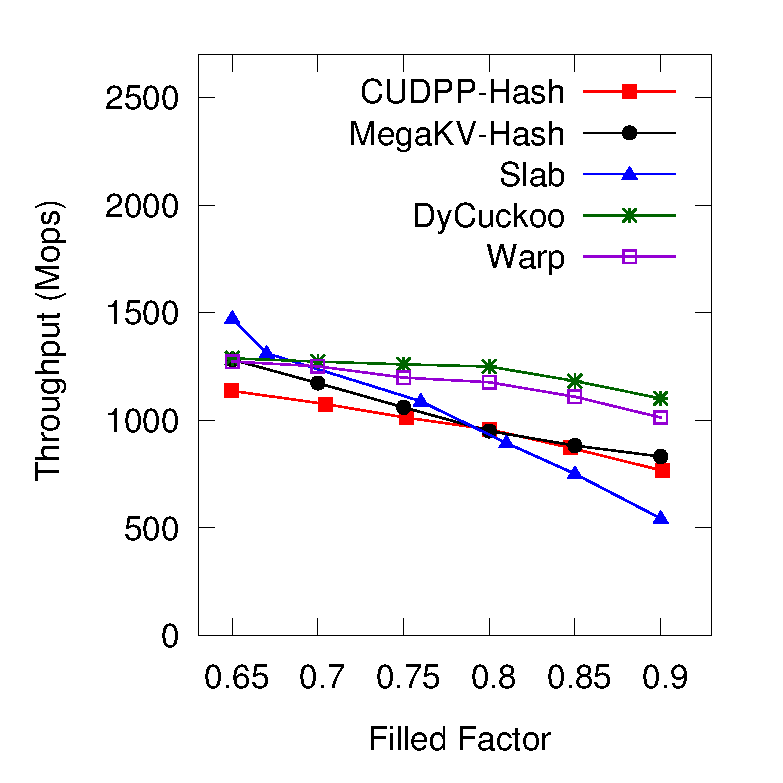
\includegraphics[width=\linewidth]{../pic/static-load_factor/ali/insert.eps}
		\centerline{\formal{insert}}
	\end{minipage}
	\hfill
	\begin{minipage}{0.48\linewidth}\centering
		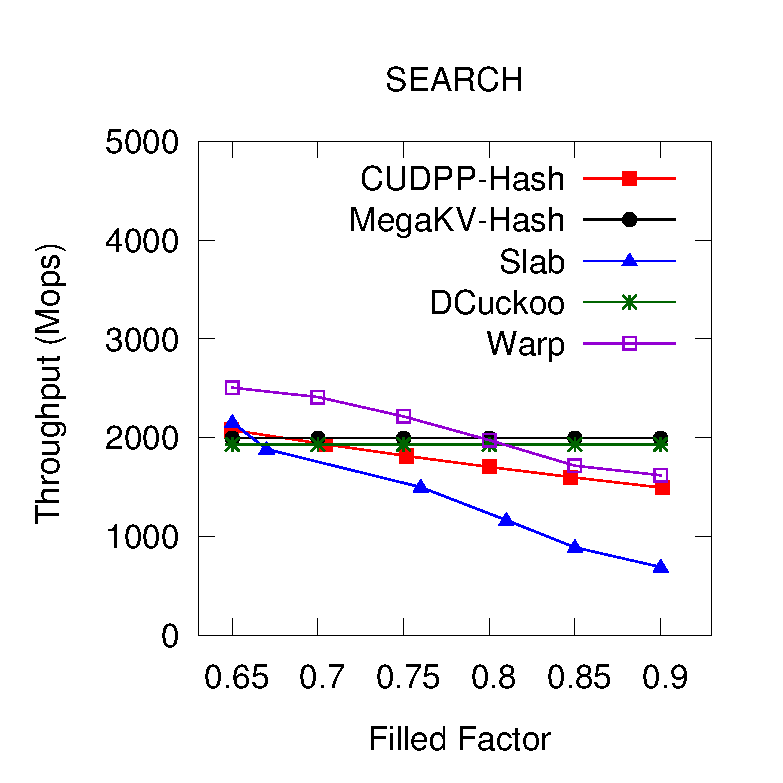
\includegraphics[width=\linewidth]{../pic/static-load_factor/ali/search.eps}
		\centerline{\formal{find}}
	\end{minipage}
	\caption{Throughput of all compared approaches for varying the filled factor against the \dsali dataset.}
	\label{fig:static-filled-factor}
\end{figure}

\begin{figure}[h]
	\begin{minipage}{0.48\linewidth}\centering
		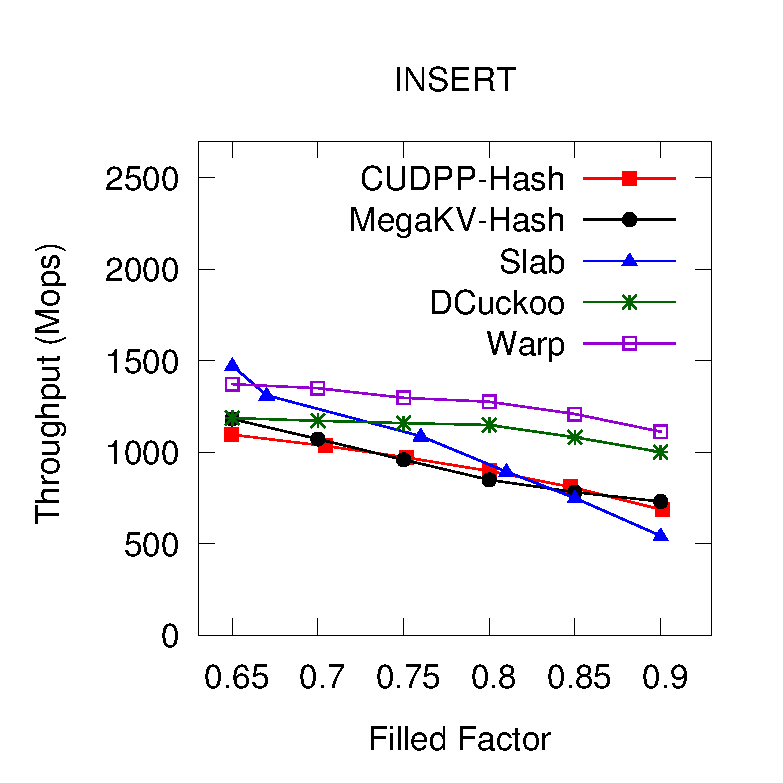
\includegraphics[width=\linewidth]{../pic/static-load_factor/reddit/insert.eps}
		\centerline{\formal{insert}}
	\end{minipage}
	\hfill
	\begin{minipage}{0.48\linewidth}\centering
		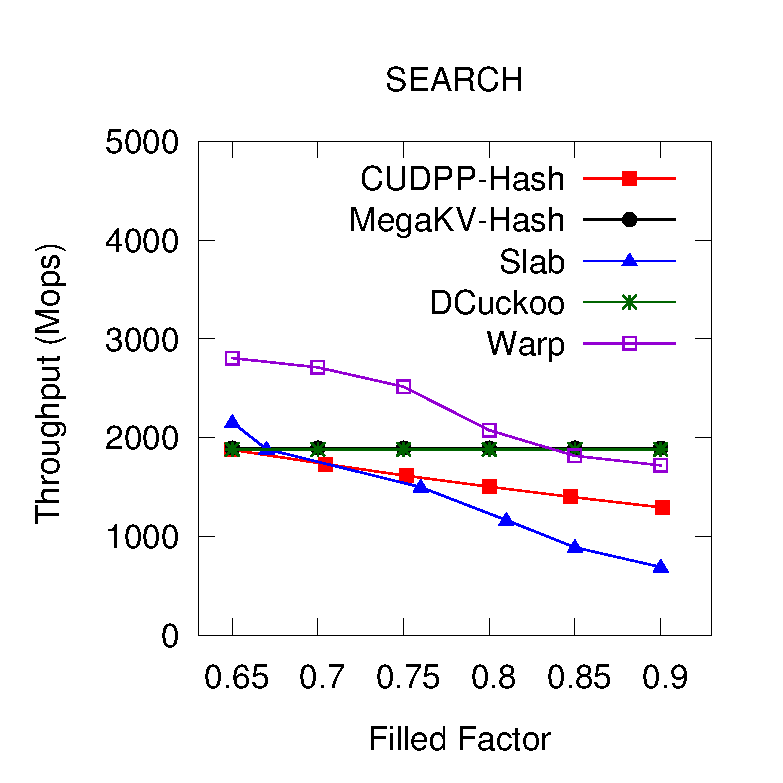
\includegraphics[width=\linewidth]{../pic/static-load_factor/reddit/search.eps}
		\centerline{\formal{find}}
	\end{minipage}
	\caption{Throughput of all compared approaches for varying the filled factor against the \dsreddit dataset.}
	\label{fig:static-filled-factor}
\end{figure}

\begin{figure}[h]
	\begin{minipage}{0.48\linewidth}\centering
		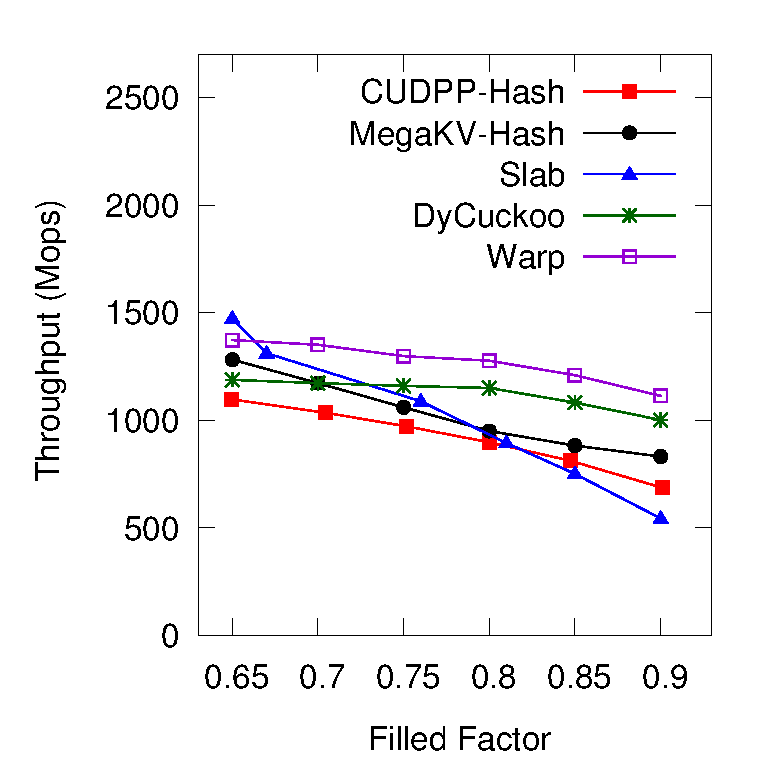
\includegraphics[width=\linewidth]{../pic/static-load_factor/twitter/insert.eps}
		\centerline{\formal{insert}}
	\end{minipage}
	\hfill
	\begin{minipage}{0.48\linewidth}\centering
		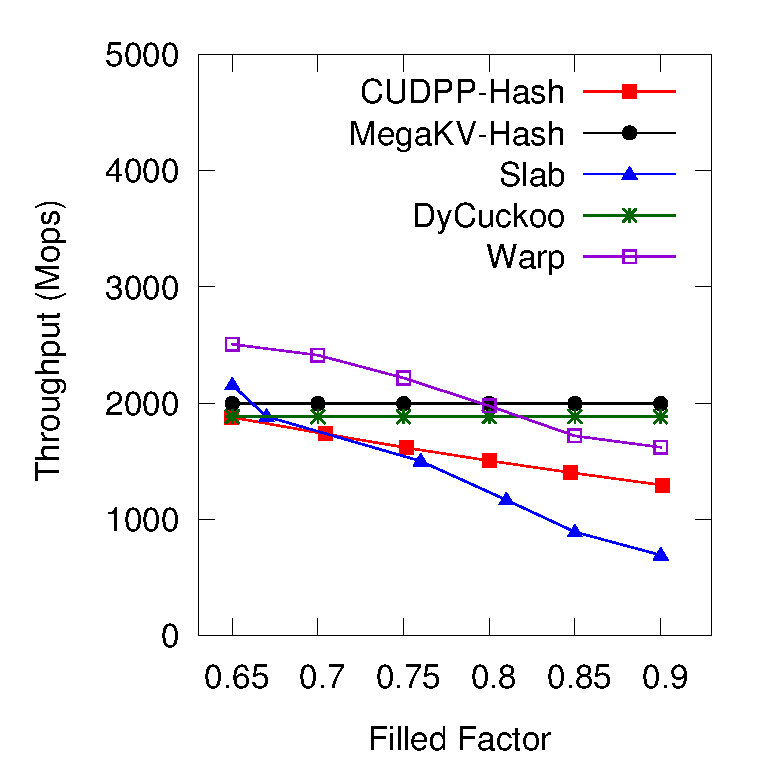
\includegraphics[width=\linewidth]{../pic/static-load_factor/twitter/search.eps}
		\centerline{\formal{find}}
	\end{minipage}
	\caption{Throughput of all compared approaches for varying the filled factor against the \dstwitter dataset.}
	\label{fig:static-filled-factor}
\end{figure}

\begin{figure}[h]
	\begin{minipage}{0.48\linewidth}\centering
		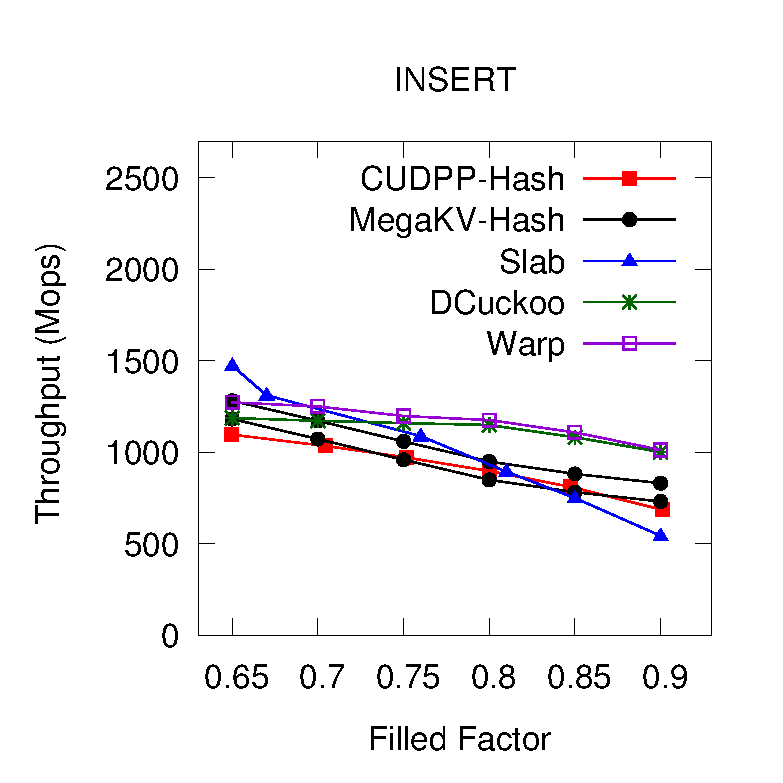
\includegraphics[width=\linewidth]{../pic/static-load_factor/tpch/insert.eps}
		\centerline{\formal{insert}}
	\end{minipage}
	\hfill
	\begin{minipage}{0.48\linewidth}\centering
		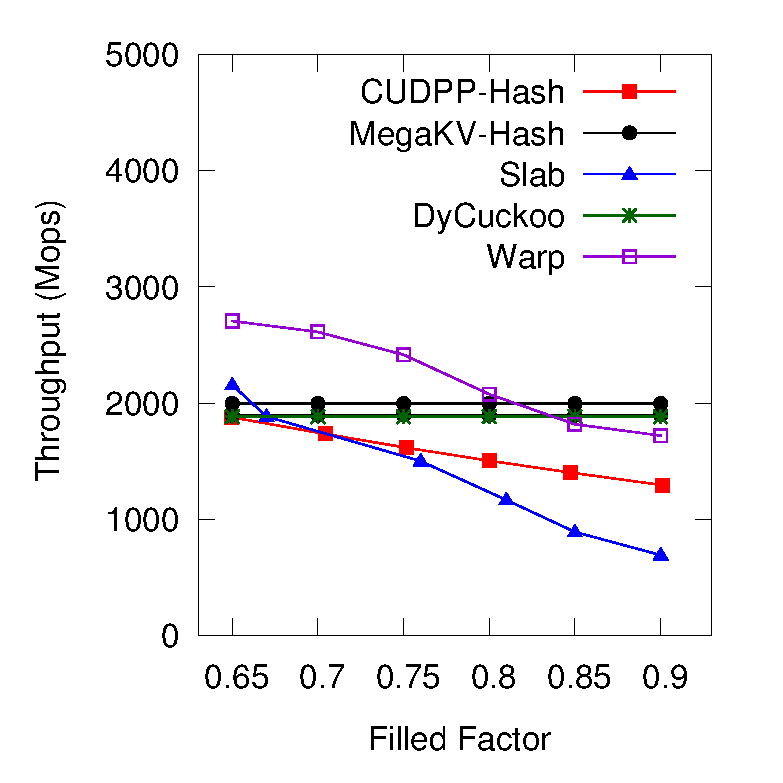
\includegraphics[width=\linewidth]{../pic/static-load_factor/tpch/search.eps}
		\centerline{\formal{find}}
	\end{minipage}
	\caption{Throughput of all compared approaches for varying the filled factor against the \dstpch dataset.}
	\label{fig:static-filled-factor}
\end{figure}
\fi

\begin{figure*}[htp]
	\begin{minipage}{0.19\linewidth}\centering
		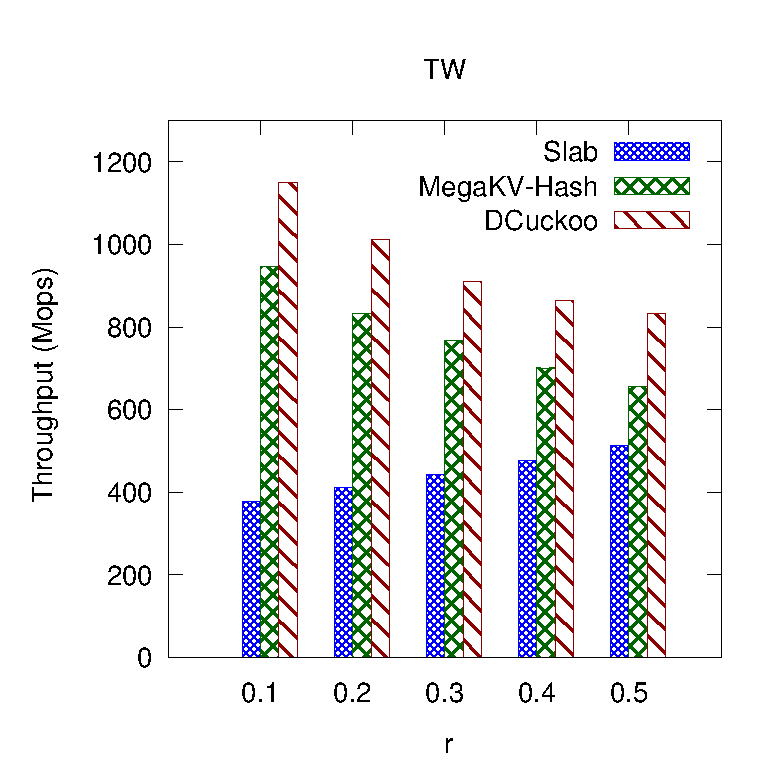
\includegraphics[width=\linewidth]{pic/dynamic/r/dynamic_twitter.eps}
		\centerline{\dstwitter}
	\end{minipage}
	\begin{minipage}{0.19\linewidth}\centering
		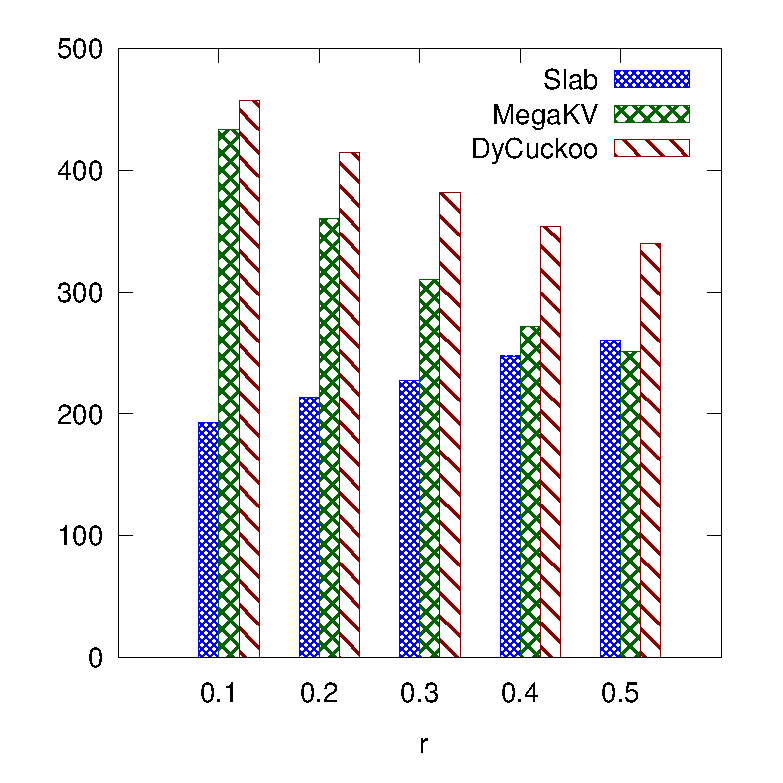
\includegraphics[width=\linewidth]{pic/dynamic/r/dynamic_reddit.eps}
		\centerline{\dsreddit}
	\end{minipage}
	\begin{minipage}{0.19\linewidth}\centering
		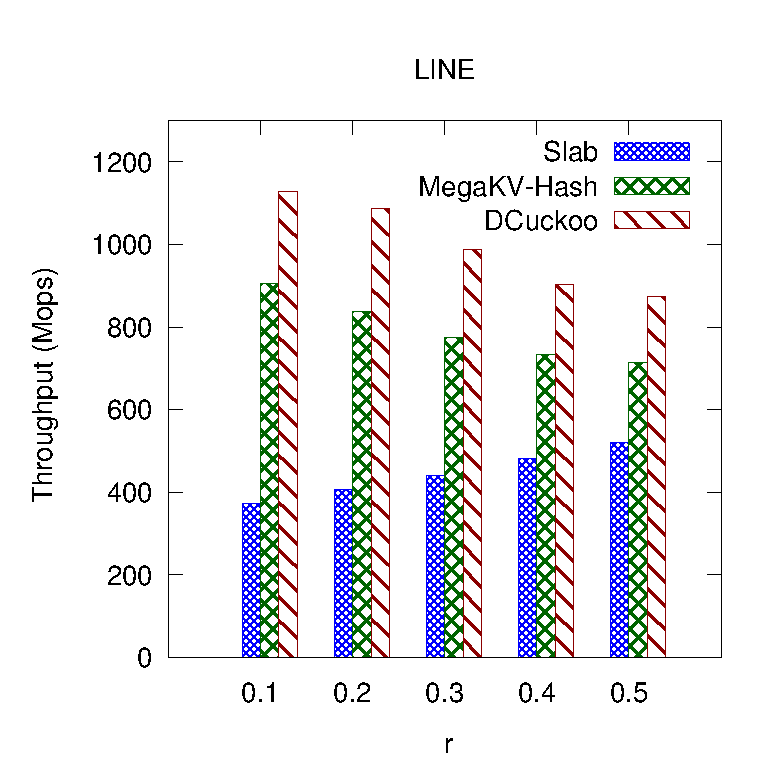
\includegraphics[width=\linewidth]{pic/dynamic/r/dynamic_tpch.eps}
		\centerline{\dstpch}
	\end{minipage}
	\begin{minipage}{0.19\linewidth}\centering
		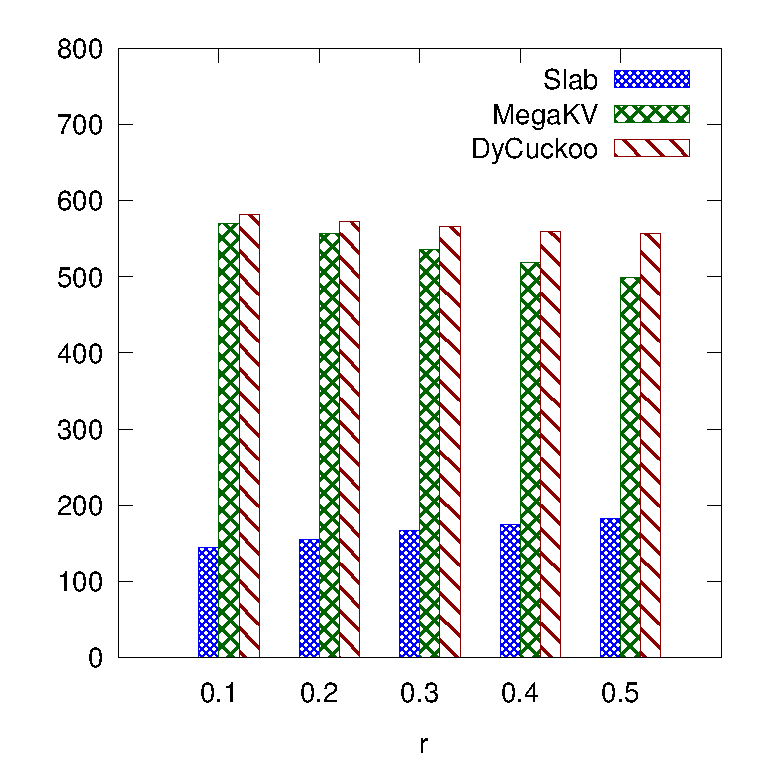
\includegraphics[width=\linewidth]{pic/dynamic/r/dynamic_ali.eps}
		\centerline{\dsali}
	\end{minipage}
	\begin{minipage}{0.19\linewidth}\centering
		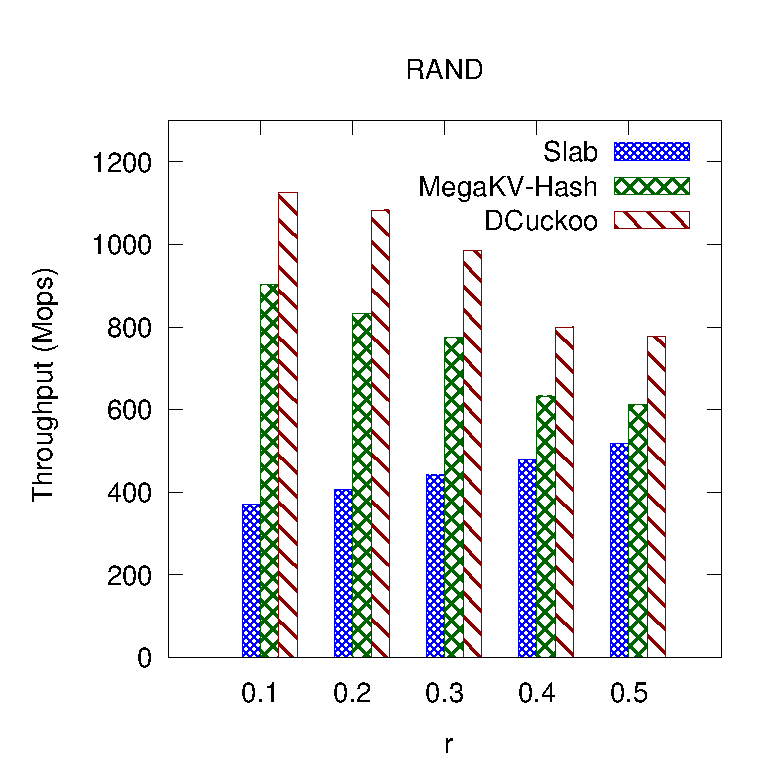
\includegraphics[width=\linewidth]{pic/dynamic/r/dynamic_random.eps}
		\centerline{\dsrandom}
	\end{minipage}
	\caption{\revise{Throughput for varying the ratio $r$.}}
	\label{fig:vary-r-time}
\end{figure*}
%
\begin{figure*}[htp]
	\begin{minipage}{0.19\linewidth}\centering
		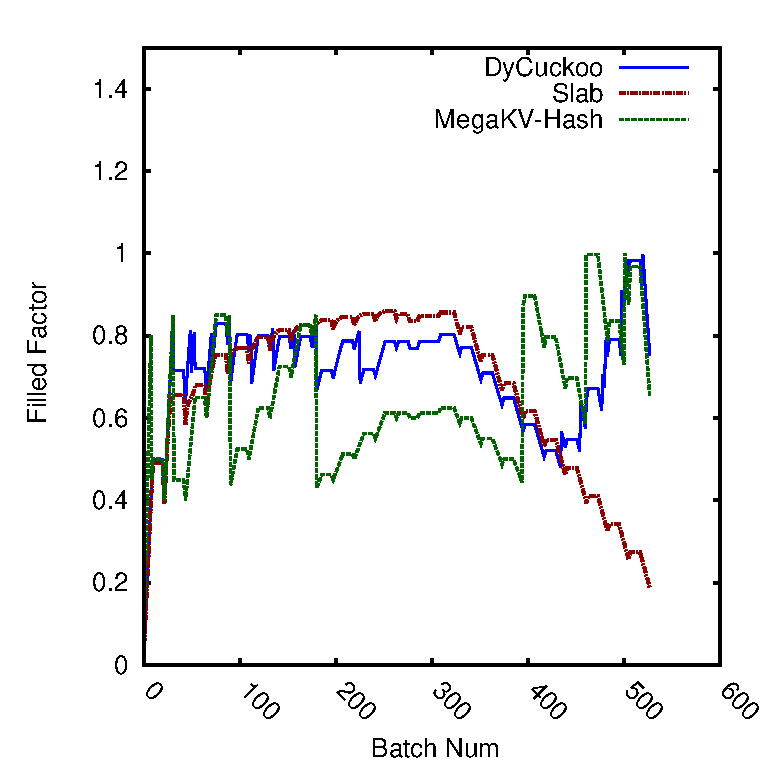
\includegraphics[width=\linewidth]{pic/dynamic-load_factor/twitter/batch_LoadFactor-2.eps}
		\centerline{\dstwitter}
	\end{minipage}
	\begin{minipage}{0.19\linewidth}\centering
		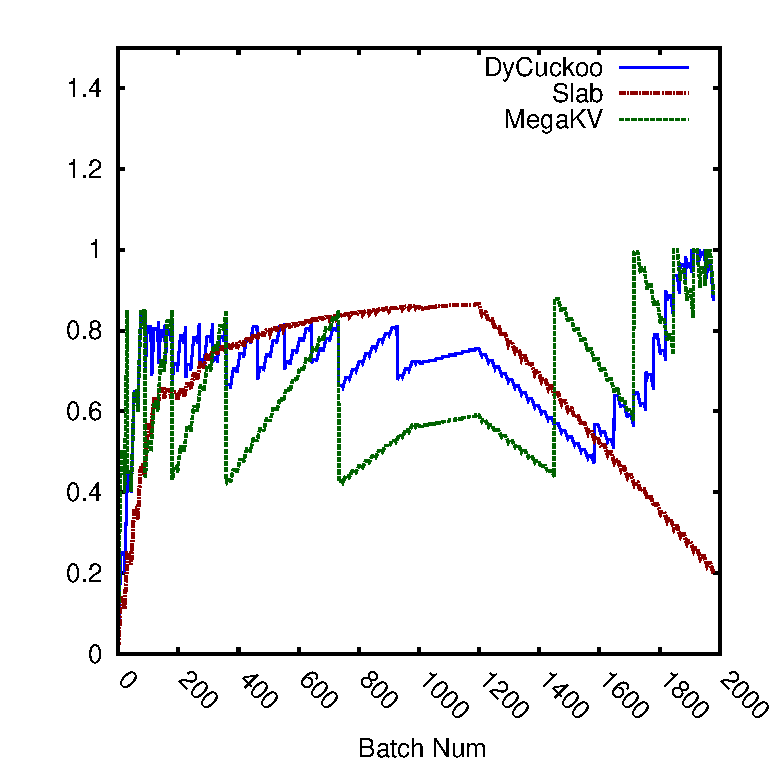
\includegraphics[width=\linewidth]{pic/dynamic-load_factor/reddit/batch_LoadFactor-2.eps}
		\centerline{\dsreddit}
	\end{minipage}
	\begin{minipage}{0.19\linewidth}\centering
		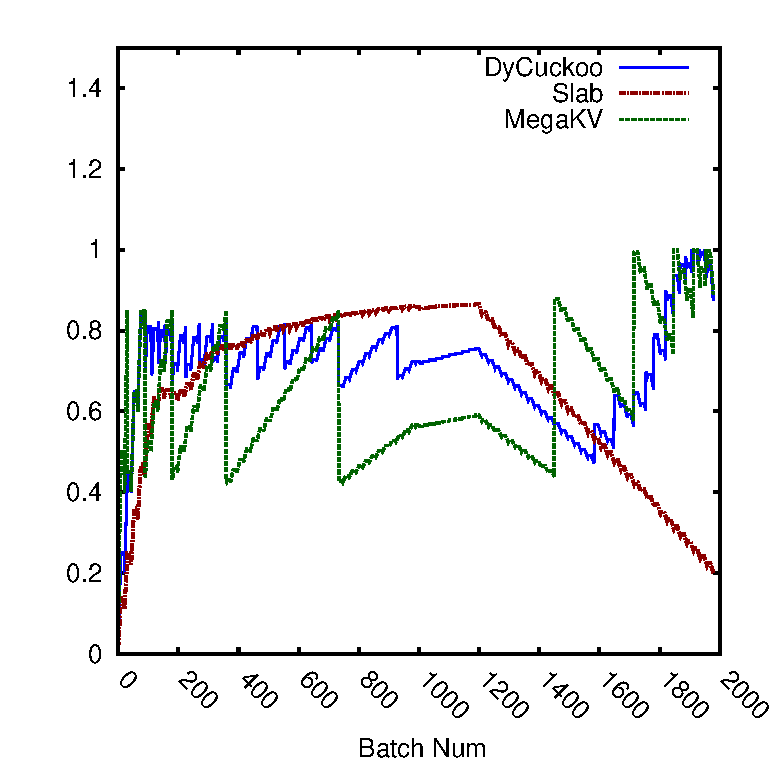
\includegraphics[width=\linewidth]{pic/dynamic-load_factor/tpch/batch_LoadFactor-2.eps}
		\centerline{\dstpch}
	\end{minipage}
	\begin{minipage}{0.19\linewidth}\centering
		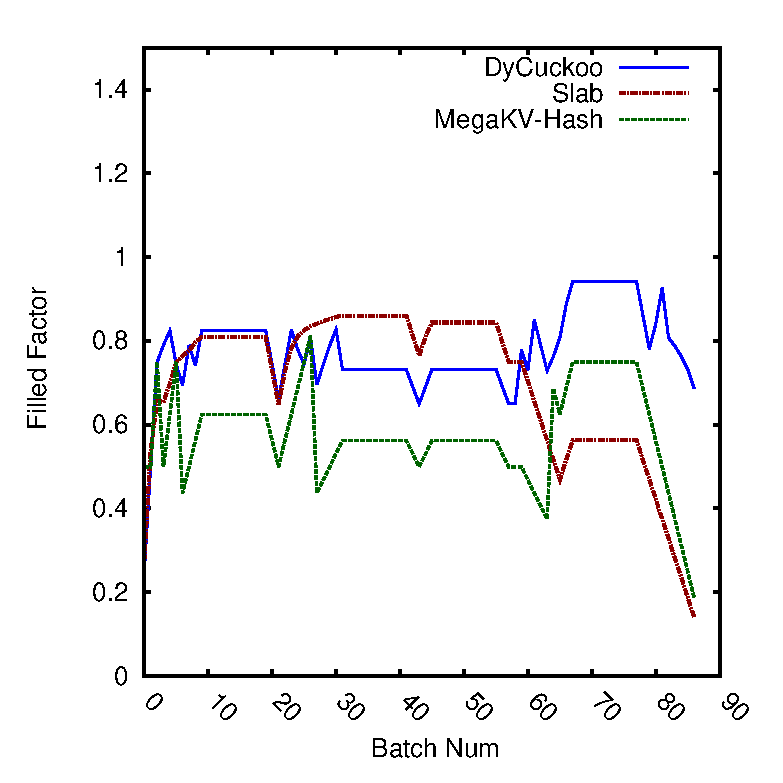
\includegraphics[width=\linewidth]{pic/dynamic-load_factor/ali/batch_LoadFactor-2.eps}
		\centerline{\dsali}
	\end{minipage}
	\begin{minipage}{0.19\linewidth}\centering
		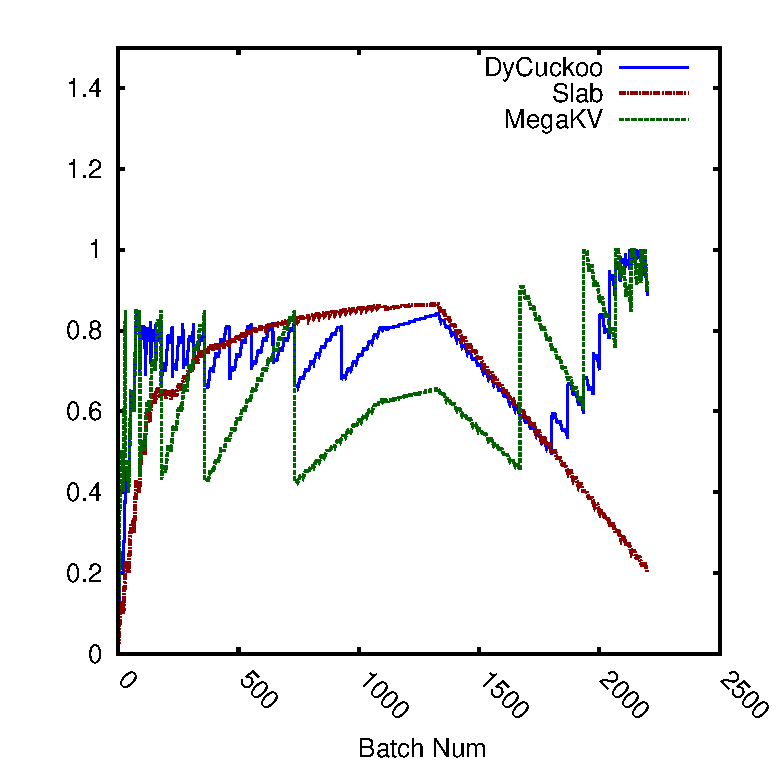
\includegraphics[width=\linewidth]{pic/dynamic-load_factor/random/batch_LoadFactor-2.eps}
		\centerline{\dsrandom}
	\end{minipage}
	\caption{\revise{Tracking the filled factor.}}
	\label{fig:track-stability}
\end{figure*}
%
\begin{figure*}[htp]
	\begin{minipage}{0.19\linewidth}\centering
		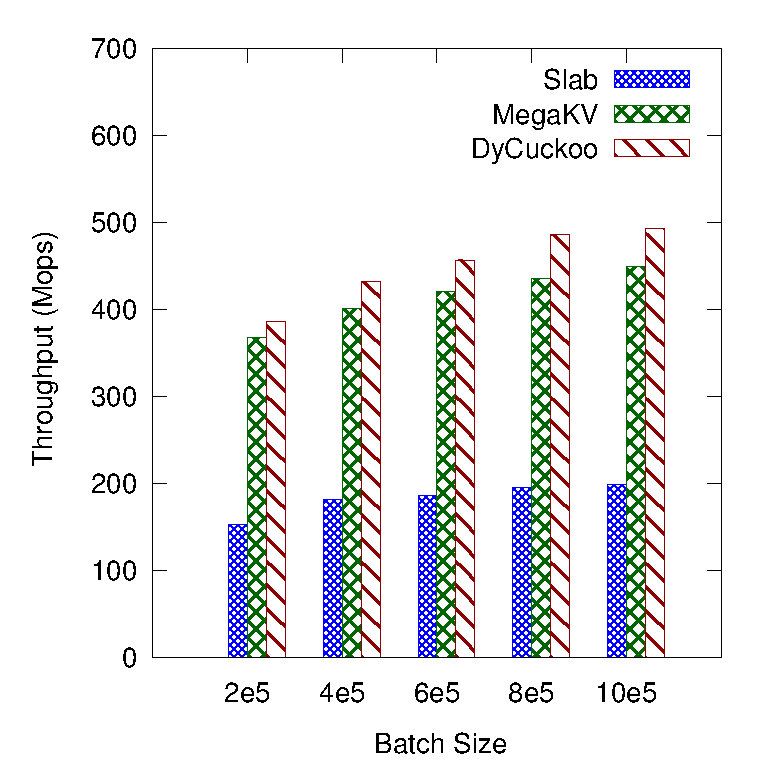
\includegraphics[width=\linewidth]{pic/dynamic/batch/dynamic_twitter.eps}
		\centerline{\dstwitter}
	\end{minipage}
	\begin{minipage}{0.19\linewidth}\centering
		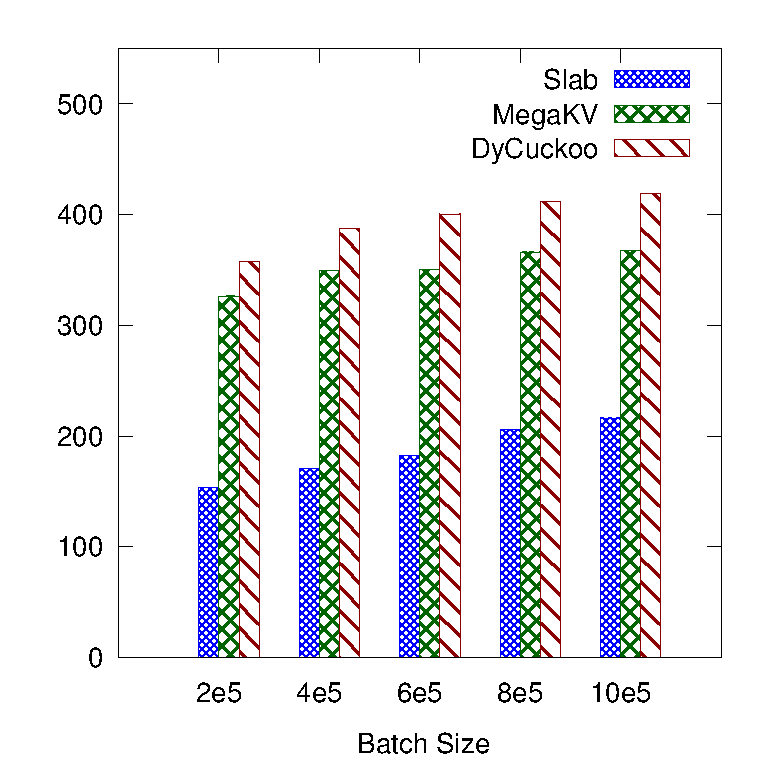
\includegraphics[width=\linewidth]{pic/dynamic/batch/dynamic_reddit.eps}
		\centerline{\dsreddit}
	\end{minipage}
	\begin{minipage}{0.19\linewidth}\centering
		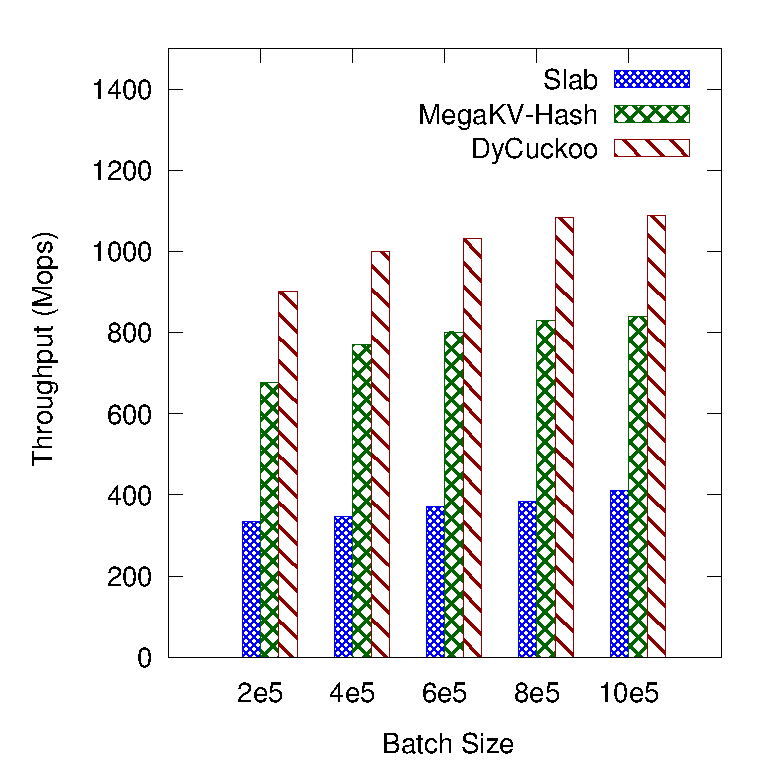
\includegraphics[width=\linewidth]{pic/dynamic/batch/dynamic_tpch.eps}
		\centerline{\dstpch}
	\end{minipage}
	\begin{minipage}{0.19\linewidth}\centering
		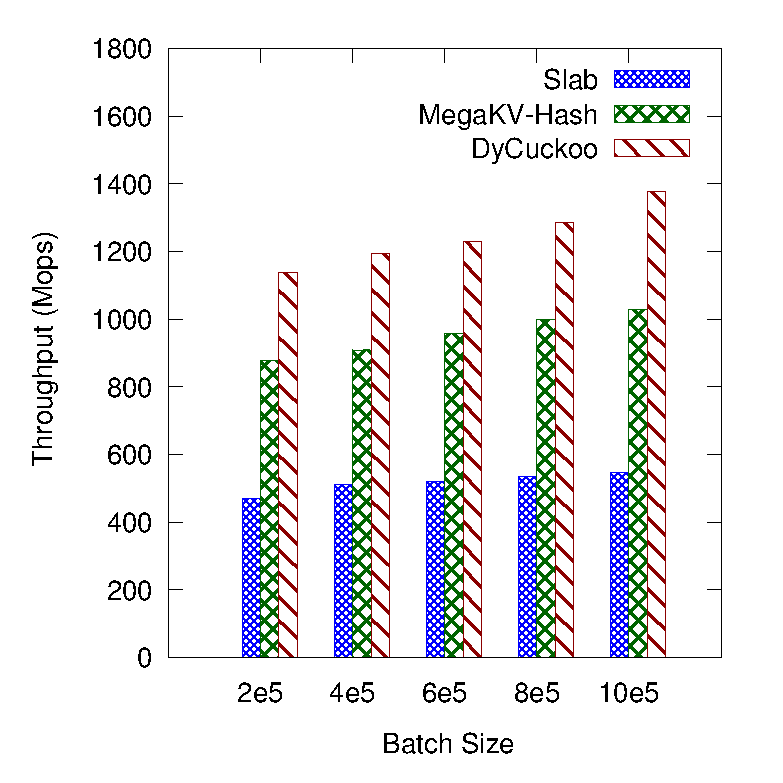
\includegraphics[width=\linewidth]{pic/dynamic/batch/dynamic_ali.eps}
		\centerline{\dsali}
	\end{minipage}
	\begin{minipage}{0.19\linewidth}\centering
		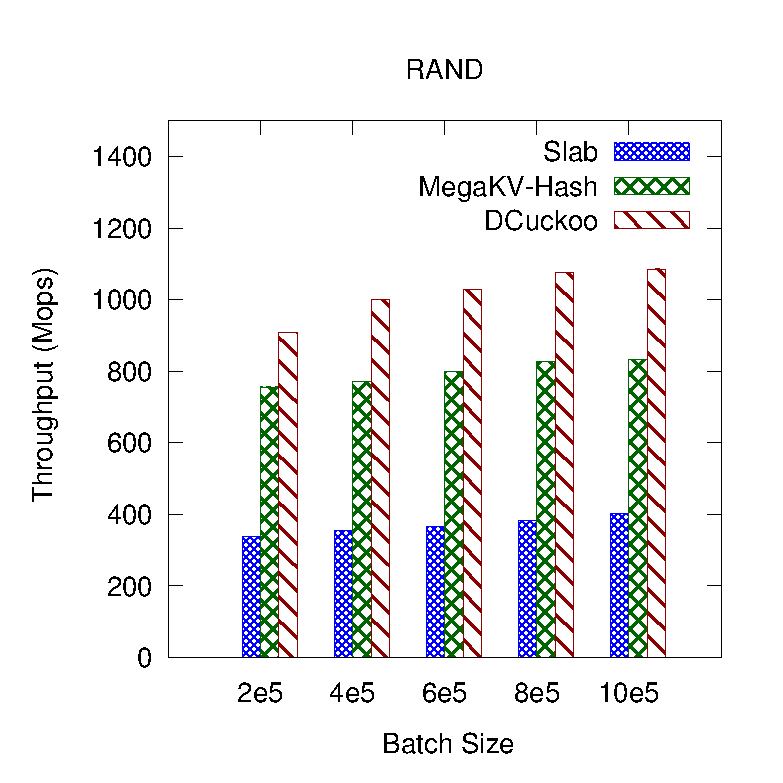
\includegraphics[width=\linewidth]{pic/dynamic/batch/dynamic_random.eps}
		\centerline{\dsrandom}
	\end{minipage}
	\caption{\revise{Throughput for varying Batch Size .}}
	\label{fig:vary-batch-size}
\end{figure*}

\subsection{Static Hashing Comparison}\label{sec:exp:static}

\vspace{1mm}\noindent\textbf{Throughput Analysis.} In Figure~\ref{fig:static-all} shows the throughput of all compared approaches over all datasets under default settings.
\revise{The GPU-based approaches outperform the CPU-based baseline with a wide margin. For \formal{insert}, \warp demonstrates the best performance overall, because \warp employs a linear probing strategy that achieves better cache locality than the cuckoo strategy \cite{junger2018warpdrive}. Nevertheless, \voter shows competitive throughput. 
For \formal{find}, \megakv shows the best performance at the default filled factor since it simply checks two buckets for locating a KV pair.
Although \voter also checks two buckets, it has slightly inferior performance to \megakv because \voter employs another layer of hashing that adds cost to the overall performance.
\slab employs a chaining approach; therefore it requires more random accesses to locate a KV pair along the chain when a high filled factor is required. Hence, \slab has inferior performance to other GPU-based solutions.}



\vspace{1mm}\noindent\textbf{Varying filled factor $\theta$.}
We vary the filled factor $\theta$ and show the performance of all GPU-based approaches against the \dsrandom dataset in Figure~\ref{fig:static-filled-factor}. The other datasets show similar trends, thus we omit those results in this paper.
\revise{For \slab, the filled factor dramatically affects the performance of both \formal{insert} and \formal{find}. This is because \slab employs a chaining approach, in which a high filled factor leads to long chains and poor performance.
Overall, \warp demonstrates superior performance for the static setting. As previously mentioned, \warp has better cache locality than the other approaches. 
\voter shows competitive performance and could even outperform \warp for high filled factors, e.g., $\theta \geq 0.85$. Furthermore, the linear probing strategy \warp adopts may need to scan multiple memory positions for \formal{find} and \formal{delete}. Although \cudpp also employs the cuckoo strategy, it automatically determines the number of hash tables for a given data size. At high filled factors, \cudpp employs more hash tables and scans more buckets; hence, its performance decreases for high filled factors. In contrast, \voter and \megakv use the cuckoo strategy and only inspect two buckets, which explains the stable throughput shown in Figure~\ref{fig:static-filled-factor} for \formal{find}. Furthermore, \voter shows better insertion performance than \megakv because our proposed strategy efficiently resolves conflicts.}



%\vspace{1mm}\noindent\textbf{GPU Profiling.} To further study the behavior of the approaches, we present three types of profiling results for all \formal{insert} GPU kernels in Figure~\ref{fig:static:profile}.
%For \emph{warp efficiency}, \voter maintains a stable rate at around 70\%, which is significantly higher than the other two cuckoo hash approaches: \megakv and \cudpp.  
%We attribute this phenomenon to the voter mechanism proposed in Section~\ref{sec:vot:con}, which yields better overall load balancing. 
%\linear could achieve higher warp efficiency than \voter, but is very volatile across different datasets. This is because each \formal{insert} in \linear may require scanning varying number of hash values for distinct data distributions. 
%For example, in the \dsali dataset, its warp efficiency drops below 40\% since \dsali contains more duplicated keys than other datasets. 

%Looking at \emph{cache} and \emph{memory bandwidth} profiling results, \megakv and \voter demonstrate better utilization as they employ the bucket mechanism.
%As \voter always needs to use atomicCAS to lock a bucket before accessing it, its utilization is inferior than that of \megakv due to the additional IO when inserting a KV pair to a bucket. In addition, atomicCAS is less efficient than atomicExch as it involves more workload per operation (see Table~\ref{fig:atomic}). Nevertheless, implementations based on atomicExch only supports KV pair with 64 bits, whereas adopting atomicCAS in \voter can support arbitrary length as we lock the bucket for exclusive update.
%It is also noted that, even though \megakv has great cache utilization due to the use of atomicExch accessing buckets directly, the overall performance is eventually bounded by device memory IOs. 

%In summary, under the static environment, \voter achieves competitive efficiency against the compared GPU baselines. Moreover, although \voter does not deliver the best performance over existing approaches, it has very low insertion failure rate and supports more general hash tables.


%





\begin{figure*}[htp]
	\begin{minipage}{0.19\linewidth}\centering
		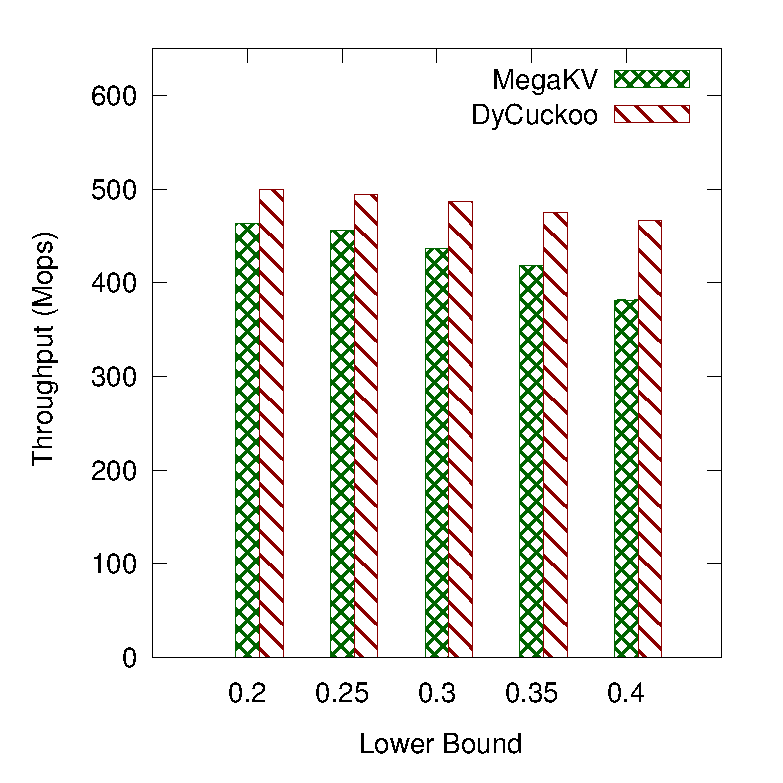
\includegraphics[width=\linewidth]{pic/dynamic/lower/dynamic_twitter.eps}
		\centerline{\dstwitter}
	\end{minipage}
	\begin{minipage}{0.19\linewidth}\centering
		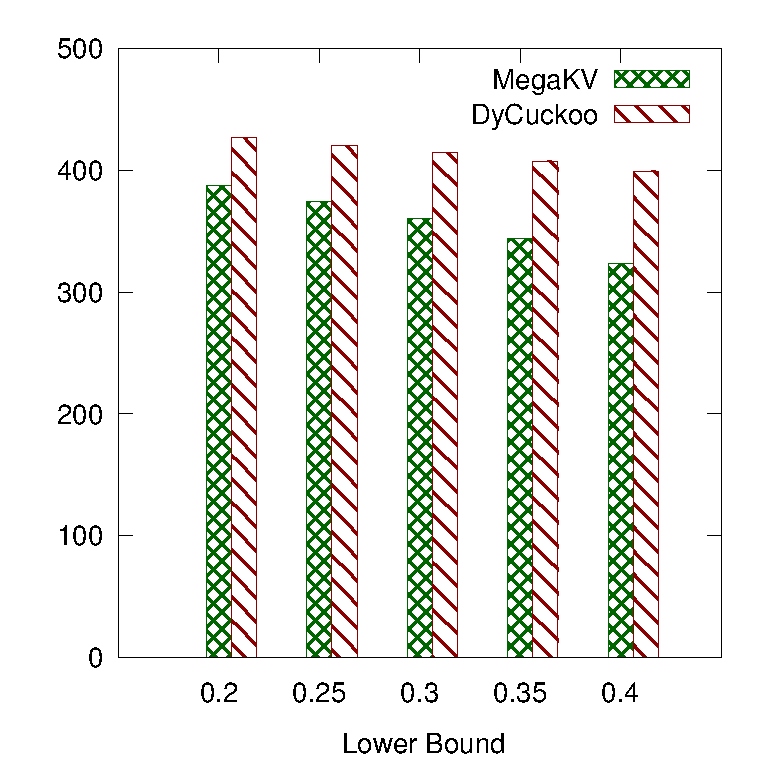
\includegraphics[width=\linewidth]{pic/dynamic/lower/dynamic_reddit.eps}
		\centerline{\dsreddit}
	\end{minipage}
	\begin{minipage}{0.19\linewidth}\centering
		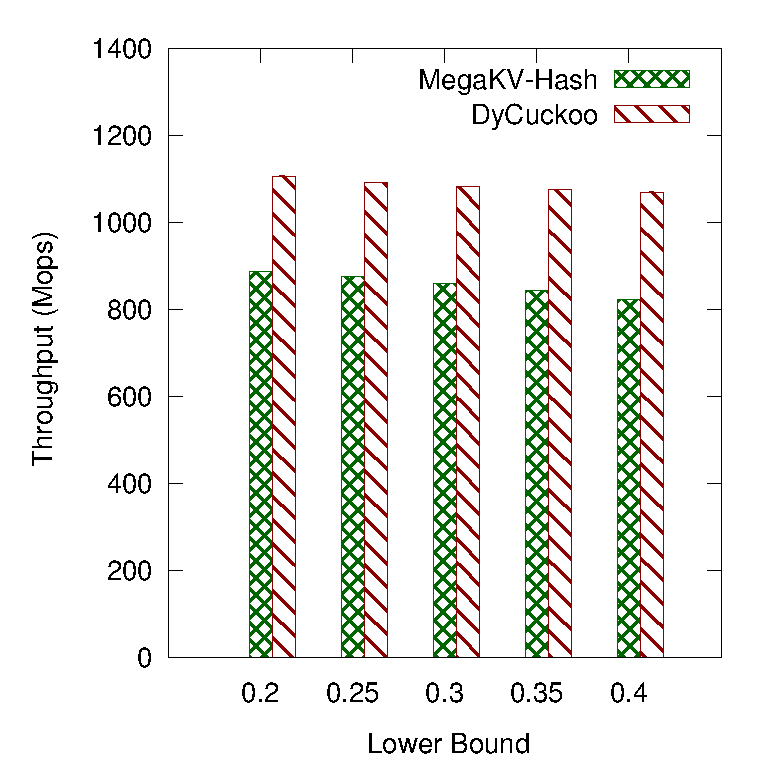
\includegraphics[width=\linewidth]{pic/dynamic/lower/dynamic_tpch.eps}
		\centerline{\dstpch}
	\end{minipage}
	\begin{minipage}{0.19\linewidth}\centering
		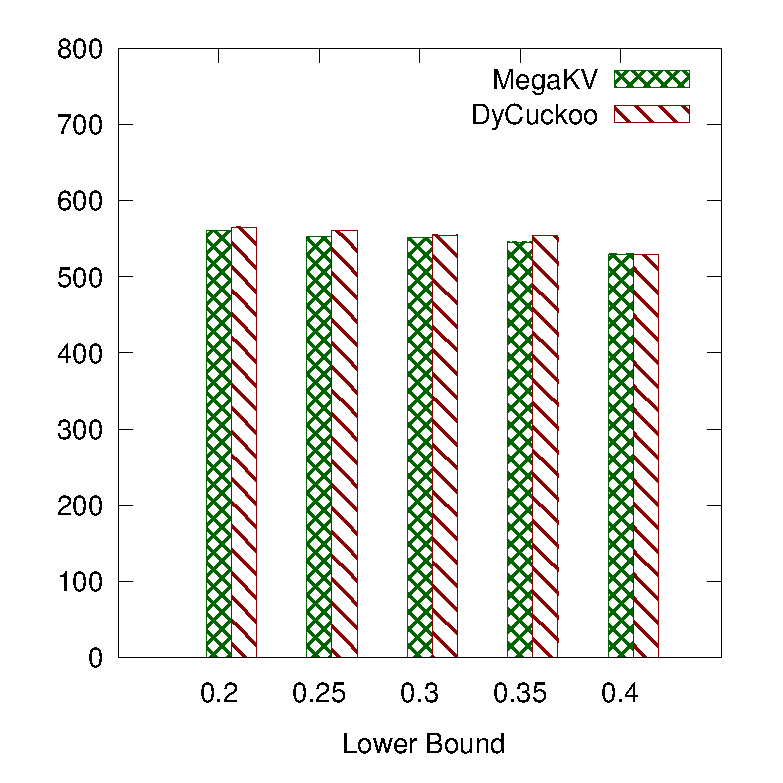
\includegraphics[width=\linewidth]{pic/dynamic/lower/dynamic_ali.eps}
		\centerline{\dsali}
	\end{minipage}
	\begin{minipage}{0.19\linewidth}\centering
		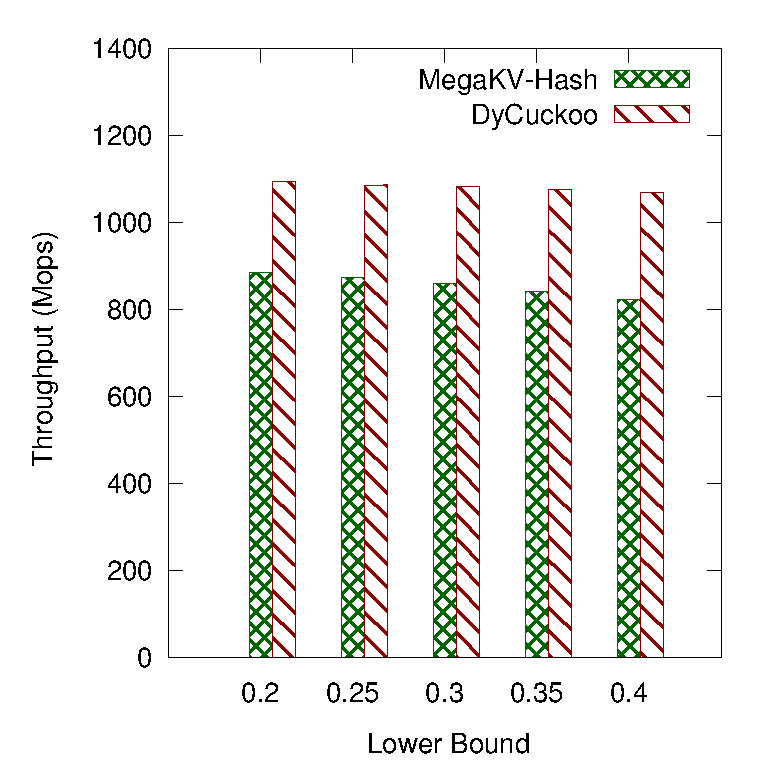
\includegraphics[width=\linewidth]{pic/dynamic/lower/dynamic_random.eps}
		\centerline{\dsrandom}
	\end{minipage}
	\caption{\revise{Throughput for varying $\alpha$ .}}
	\label{fig:vary-lower-time}
\end{figure*}

\begin{figure*}[htp]
	\begin{minipage}{0.19\linewidth}\centering
		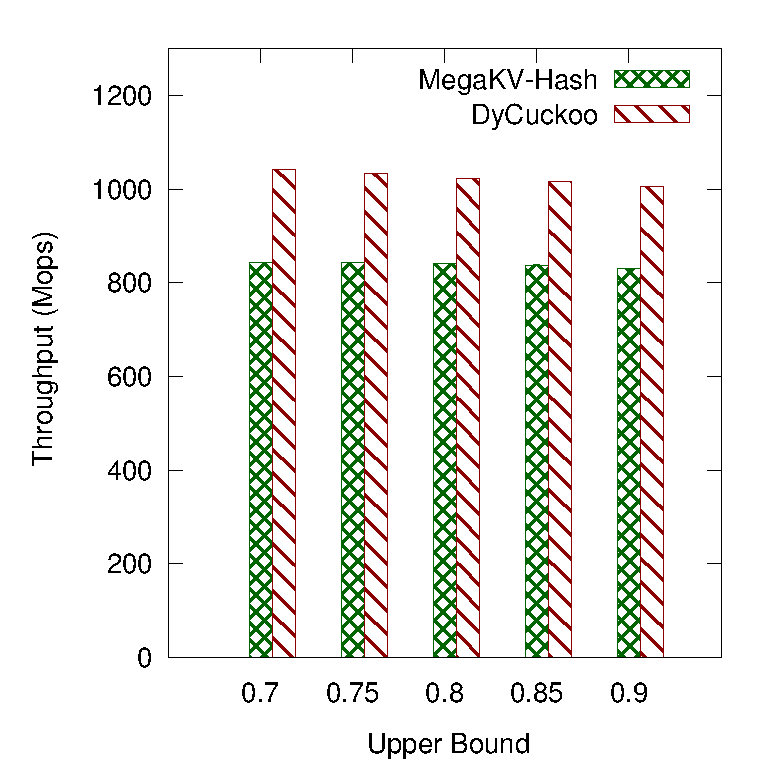
\includegraphics[width=\linewidth]{pic/dynamic/upper/dynamic_twitter.eps}
		\centerline{\dstwitter}
	\end{minipage}
	\begin{minipage}{0.19\linewidth}\centering
		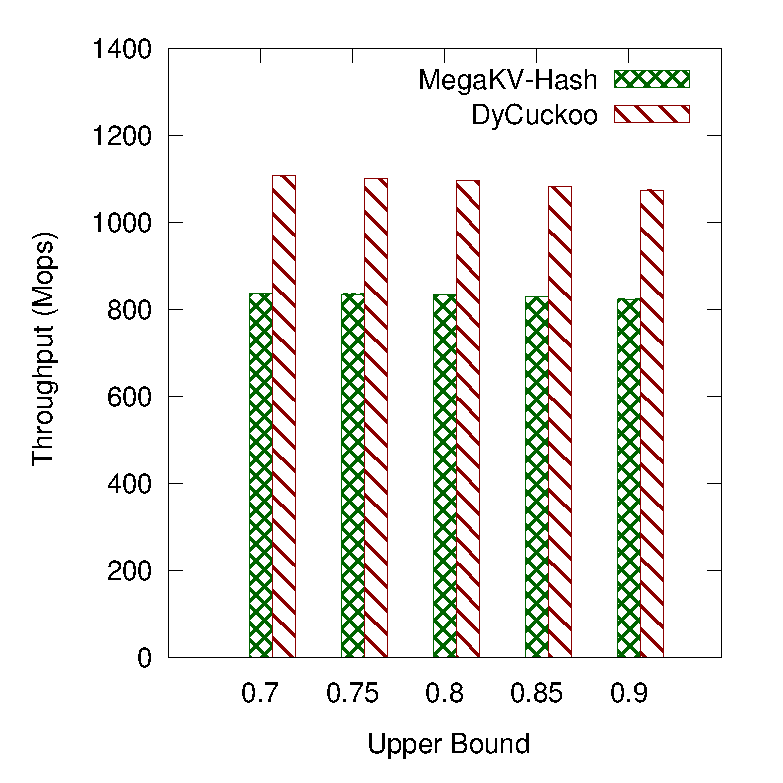
\includegraphics[width=\linewidth]{pic/dynamic/upper/dynamic_reddit.eps}
		\centerline{\dsreddit}
	\end{minipage}
	\begin{minipage}{0.19\linewidth}\centering
		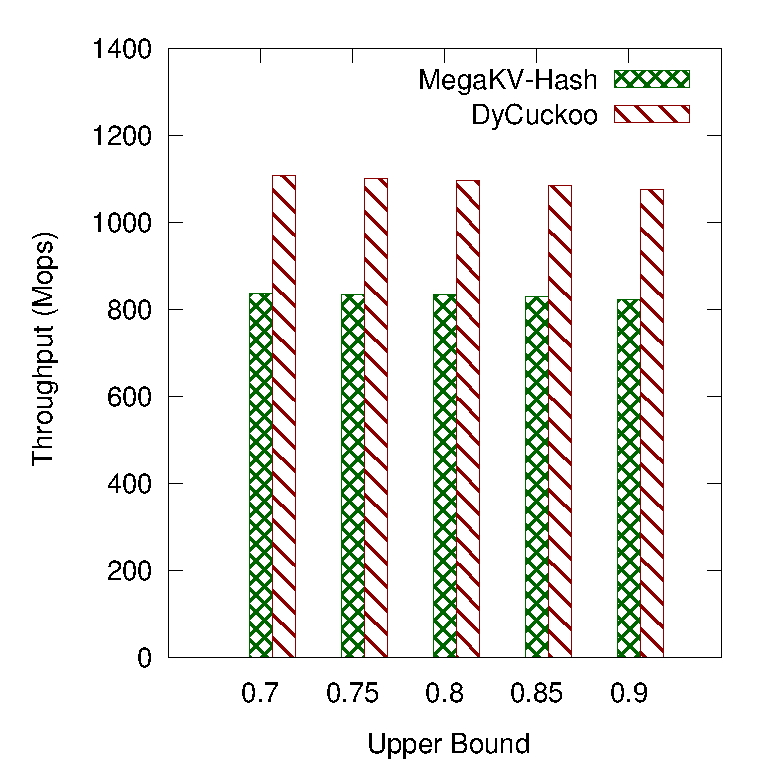
\includegraphics[width=\linewidth]{pic/dynamic/upper/dynamic_tpch.eps}
		\centerline{\dstpch}
	\end{minipage}
	\begin{minipage}{0.19\linewidth}\centering
		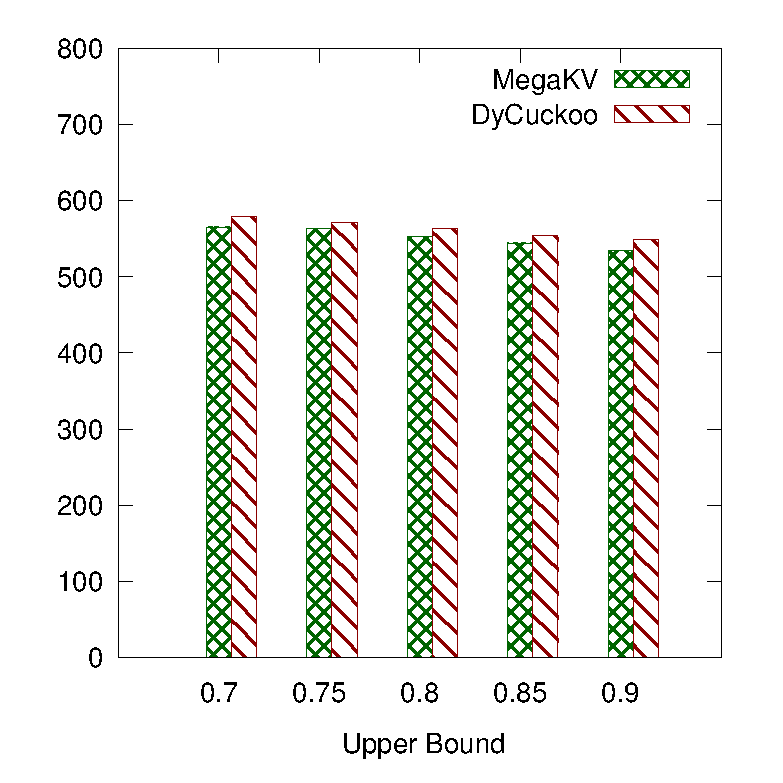
\includegraphics[width=\linewidth]{pic/dynamic/upper/dynamic_ali.eps}
		\centerline{\dsali}
	\end{minipage}
	\begin{minipage}{0.19\linewidth}\centering
		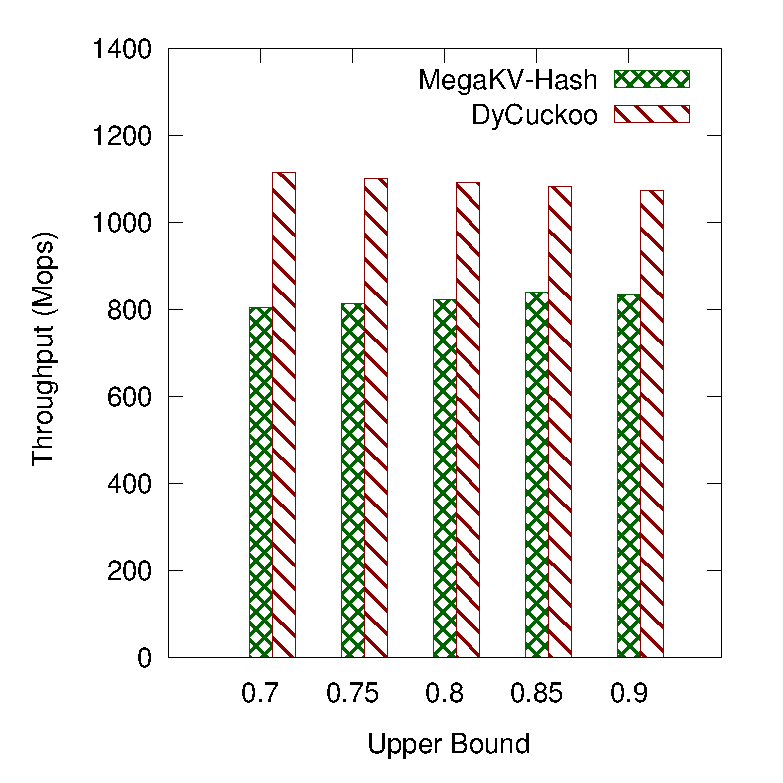
\includegraphics[width=\linewidth]{pic/dynamic/upper/dynamic_random.eps}
		\centerline{\dsrandom}
	\end{minipage}
	\caption{\revise{Throughput for varying $\beta$ .}}
	\label{fig:vary-upper-time}
\end{figure*}

\subsection{Dynamic Hashing Comparison}\label{sec:exp:dynamic}

\noindent\textbf{Varying insert vs. delete ratio $r$.}
In Figure~\ref{fig:vary-r-time}, we report the results for varying the ratio $r$, which is number of deletions over the number of insertions in a batch.
We found that for a larger value of $r$, the performance of \voter and \megakv degrades whereas that of \slab improves. A larger value of $r$ indicates more deletions, thus resizing operations are more frequently invoked for \voter and \megakv. In contrast, a greater number of deletions leads to additional vacant spaces for \slab, as that technique simply symbolically marks a deleted KV pair. Insertions are processed more efficiently for \slab because the inserted KV pairs can overwrite symbolically deleted ones. Hence, \slab utilizes more GPU device memory than \voter and \megakv. However, symbolic deletions cannot guarantee a bounded filled factor and may lead to arbitrary bad memory efficiency. This will be discussed with more experimental results later in this section.
\voter shows the best overall performance. Furthermore, the throughput margin between \voter and \megakv increases for larger $r$ values. 
As mentioned previously, a larger $r$ triggers more resizing operations, thus \voter is more efficient than \megakv as \megakv employs a total rehashing approach. 

%\linear and \megakv remains inefficient as they incur expensive overheads of resizing. An interesting observation for \linear and \megakv is that there exists a sweet spot where the resizing cost is the minimal.
%It is because the workload composition of insertions and deletions should be just right so that it does not trigger unnecessary upsizings or downsizings. However, in reality, the workloads could vary significantly and existing methods cannot be easily adapted while maintaining guaranteed filled factor. This has again validated the effectiveness of \voter against dynamic workloads.


\vspace{1mm}\noindent\textbf{Performance stability.}
We evaluate the performance stability of the compared approaches in Figure~\ref{fig:track-stability}. 
In particular, we track the filled factor after processing each batch.
\slab shows good stability in terms of memory usage for the starting phases. Unfortunately, due to the symbolic deletion approach employed, the memory efficiency of \slab degrades significantly as more deletions are processed. In particular, its filled factor drops to less than $20\%$ after processing fewer than 100 batches for the \dsali dataset, which deems a complete rebuild.
%
\megakv shows an unstable trend since it employs a simple double/half approach for resizing. We can see that its filled factor jumps up or down dramatically at resizing points. \voter demonstrates the best overall stability and saves up to 4x memory over the  compared baselines (the \dsali dataset). 
These results have validated our design, with only one of the subtables being subject to resizing. 
Nevertheless, there is still rooms for improvement. We note that for some datasets, i.e., \dstwitter, \dsreddit, \dstpch, and \dsrandom, the filled factor of \voter drops sharply.
This is because, even after upsizing one time, the insertions fail due to too many evictions, which triggers another round of upsizing. We leave this as an area for future work. 


\vspace{1mm}\noindent\textbf{Varying the batch size.}
We also varied the size of each processing batch. The results are reported in Figure~\ref{fig:vary-batch-size}. 
\slab continues to show inferior performance to \megakv and \voter. 
This is because \slab accommodates new inserted KV pairs with the chaining approach and does not increase the range of the unique hash values. Hence, a stream of insertions will eventually lead to long chains, which hurts the performance of hash table operations. Furthermore, \voter presents better performance than \megakv and the margin increases with a larger batch size.
\revise{Note that one limitation of existing GPU-based approaches is that they apply updates at the granularity of batches. It is an interesting direction for exploring efficient GPU hashing when a required update order is enforced.}


\vspace{1mm}\noindent\textbf{Varying the filled factor lower bound $\alpha$.}
We vary the lower bound of the filled factor and report the results in Figure~\ref{fig:vary-lower-time}. 
We only compare \megakv and \voter since \slab is unable to control the filled factor because of \slab's symbolic deletion approach. 
Apparently, the simple resizing strategy adopted by \megakv incurs substantial overhead. Such overhead grows for a higher $\alpha$ since the number of downsizings increases. The performance of \voter is not affected significantly due to the incremental resizing approach by updating only one subtable at a time. 
%We note that, the performance of \megakv is competitive against \voter for the \dsali dataset. This is because \megakv occupies significant more memory spaces than that of \voter, as evidenced in Figure~\ref{fig:track-stability}. Hence, \megakv trades space efficiency with time efficiency.
%Nevertheless, \voter remains superior over \megakv in terms of time efficiency while saves GPU memory substantially. 



\vspace{1mm}\noindent\textbf{Varying the filled factor upper bound $\beta$.}
The results for varying $\beta$ is reported in Figure~\ref{fig:vary-upper-time}. 
It is interesting to see that the upper bound does not significantly affect the overall performance for \megakv and \voter. 
On one hand, a higher filled factor leads to slower \formal{insert} performance. On the other hand, smaller number of rehashing is incurred for a higher filled factor. Thus, the overall performance remains stable as the opposing factors cancel each other. Nevertheless, \voter remains superior over \megakv in terms of time efficiency while saves GPU memory substantially.

%\megakv has competitive efficiency against \voter in the \dsali dataset. %The reason is similar as we discussed for varying the lower bound $\alpha$.

\iffalse
\begin{figure*}[htp]
	\begin{minipage}{0.16\linewidth}\centering
		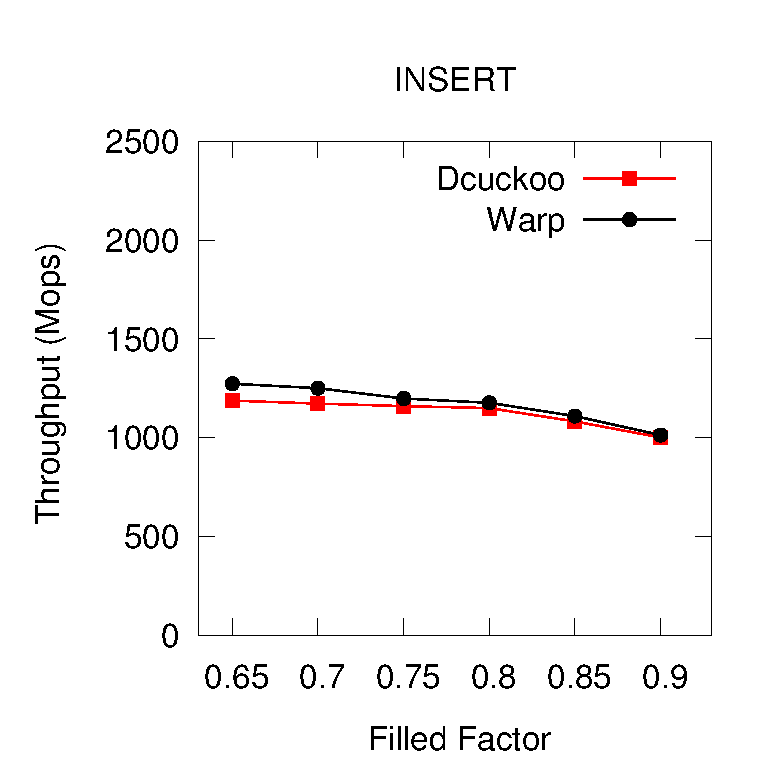
\includegraphics[width=\linewidth]{pic/group-size/g1-insert.eps}
		\centerline{group size=1}
	\end{minipage}
	\begin{minipage}{0.16\linewidth}\centering
		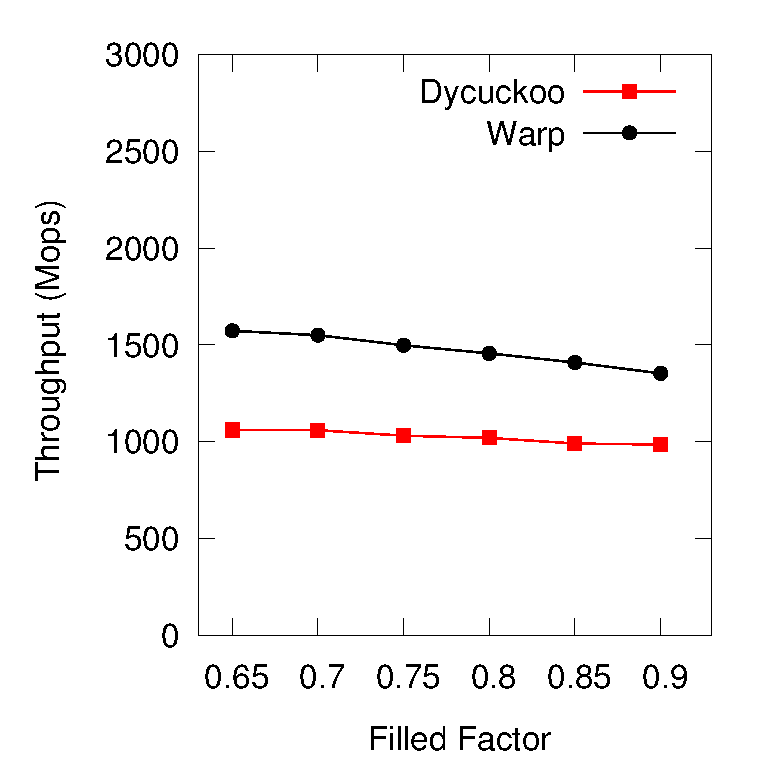
\includegraphics[width=\linewidth]{pic/group-size/g2-insert.eps}
		\centerline{group size=2}
	\end{minipage}
	\begin{minipage}{0.16\linewidth}\centering
		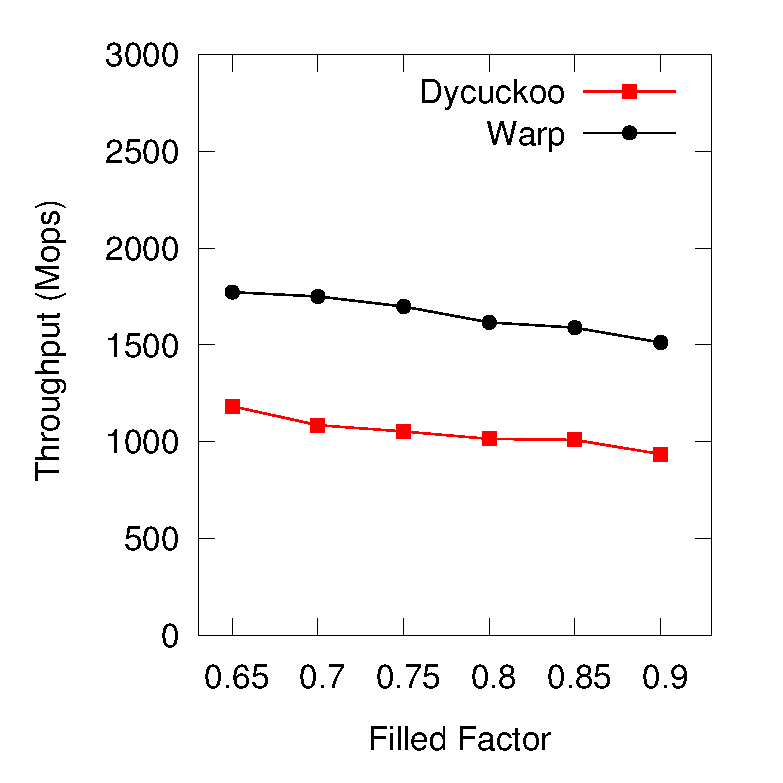
\includegraphics[width=\linewidth]{pic/group-size/g4-insert.eps}
		\centerline{group size=4}
	\end{minipage}
	\begin{minipage}{0.16\linewidth}\centering
		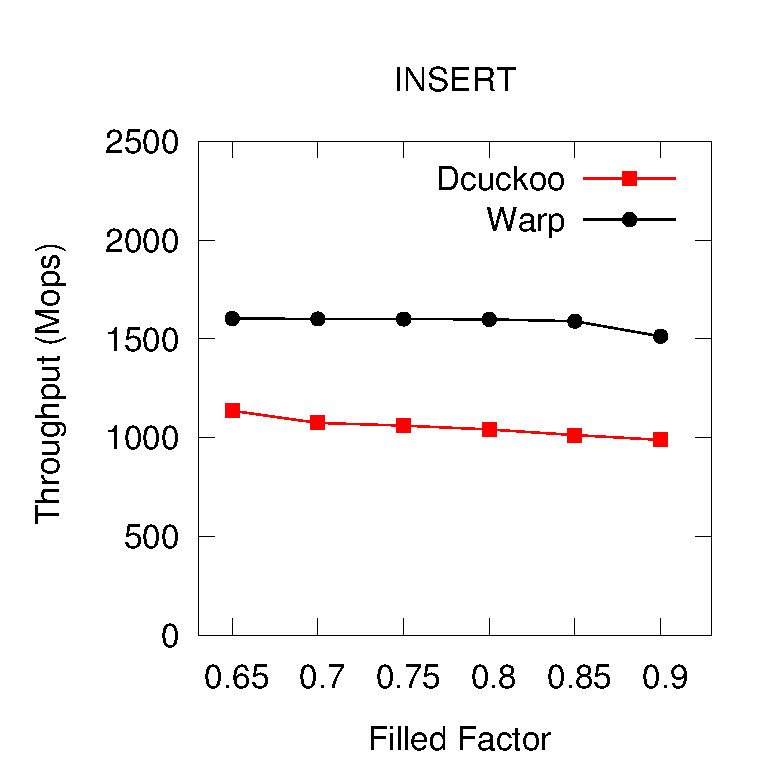
\includegraphics[width=\linewidth]{pic/group-size/g8-insert.eps}
		\centerline{group size=8}	
		\end{minipage}
	\begin{minipage}{0.16\linewidth}\centering
		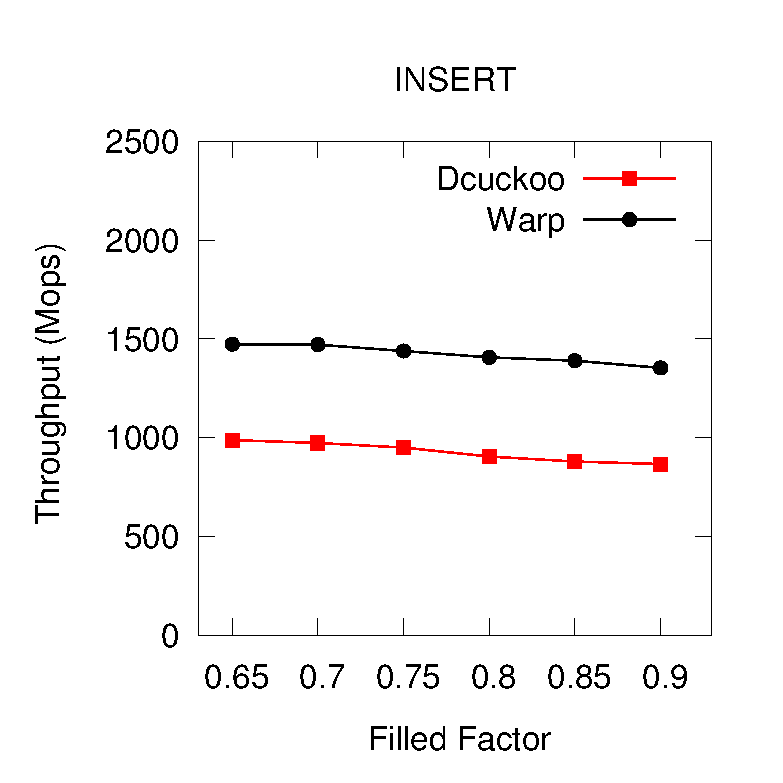
\includegraphics[width=\linewidth]{pic/group-size/g16-insert.eps}
		\centerline{group size=16}
	\end{minipage}
	\begin{minipage}{0.16\linewidth}\centering
		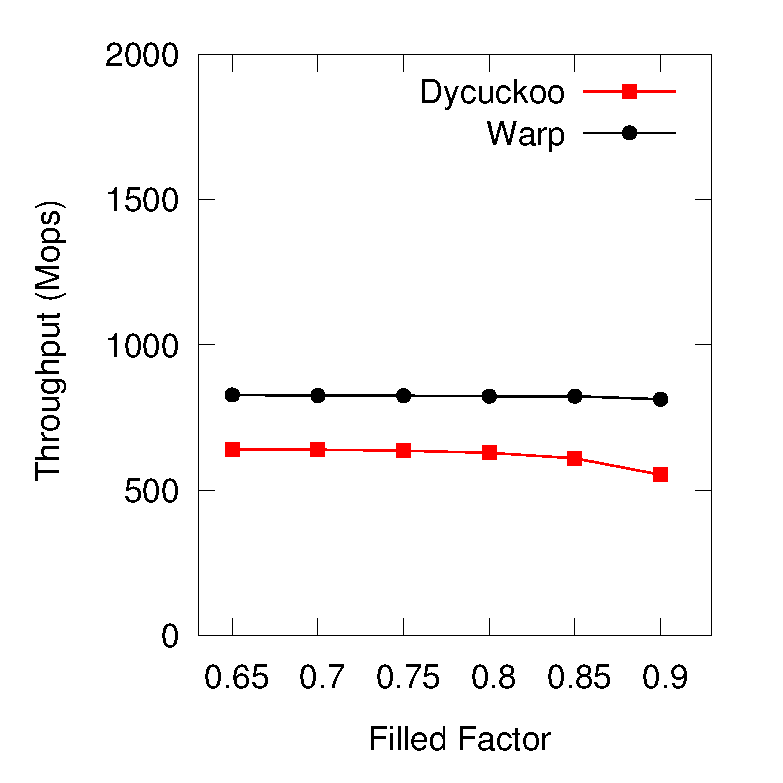
\includegraphics[width=\linewidth]{pic/group-size/g32-insert.eps}
		\centerline{group size=32}
	\end{minipage}
	\caption{Throughput of insert for varying group size .}
	\label{fig:vary-upper-time}
\end{figure*}


\begin{figure*}[htp]
	\begin{minipage}{0.16\linewidth}\centering
		\includegraphics[width=\linewidth]{pic/group-size/g1-search.eps}
		\centerline{group size=1}
	\end{minipage}
	\begin{minipage}{0.16\linewidth}\centering
		\includegraphics[width=\linewidth]{pic/group-size/g2-search.eps}
		\centerline{group size=2}
	\end{minipage}
	\begin{minipage}{0.16\linewidth}\centering
		\includegraphics[width=\linewidth]{pic/group-size/g4-search.eps}
		\centerline{group size=4}
	\end{minipage}
	\begin{minipage}{0.16\linewidth}\centering
		\includegraphics[width=\linewidth]{pic/group-size/g8-search.eps}
		\centerline{group size=8}	
		\end{minipage}
	\begin{minipage}{0.16\linewidth}\centering
		\includegraphics[width=\linewidth]{pic/group-size/g16-search.eps}
		\centerline{group size=16}
	\end{minipage}
	\begin{minipage}{0.16\linewidth}\centering
		\includegraphics[width=\linewidth]{pic/group-size/g32-search.eps}
		\centerline{group size=32}
	\end{minipage}
	\caption{Throughput of search for varying group size .}
	\label{fig:vary-upper-time}
\end{figure*}
\fi



